\documentclass[a4paper]{book}
\usepackage{makeidx}
\usepackage{graphicx}
\usepackage{multicol}
\usepackage{float}
\usepackage{listings}
\usepackage{color}
\usepackage{ifthen}
\usepackage[table]{xcolor}
\usepackage{textcomp}
\usepackage{alltt}
\usepackage{ifpdf}
\ifpdf
\usepackage[pdftex,
            pagebackref=true,
            colorlinks=true,
            linkcolor=blue,
            unicode
           ]{hyperref}
\else
\usepackage[ps2pdf,
            pagebackref=true,
            colorlinks=true,
            linkcolor=blue,
            unicode
           ]{hyperref}
\usepackage{pspicture}
\fi
\usepackage[utf8]{inputenc}
\usepackage{mathptmx}
\usepackage[scaled=.90]{helvet}
\usepackage{courier}
\usepackage{doxygen}
\lstset{language=C++,inputencoding=utf8,basicstyle=\footnotesize,breaklines=true,breakatwhitespace=true,tabsize=8,numbers=left }
\makeindex
\setcounter{tocdepth}{3}
\renewcommand{\footrulewidth}{0.4pt}
\begin{document}
\hypersetup{pageanchor=false}
\begin{titlepage}
\vspace*{7cm}
\begin{center}
{\Large Transcode \\[1ex]\large 1.0 }\\
\vspace*{1cm}
{\large Generated by Doxygen 1.7.3}\\
\vspace*{0.5cm}
{\small Sun Mar 18 2012 11:41:13}\\
\end{center}
\end{titlepage}
\clearemptydoublepage
\pagenumbering{roman}
\tableofcontents
\clearemptydoublepage
\pagenumbering{arabic}
\hypersetup{pageanchor=true}
\chapter{Namespace Index}
\section{Namespace List}
Here is a list of all documented namespaces with brief descriptions:\begin{DoxyCompactList}
\item\contentsline{section}{\hyperlink{namespacecallback}{callback} (Callback namespace, all callback functions are found here )}{\pageref{namespacecallback}}{}
\item\contentsline{section}{\hyperlink{namespacehelper}{helper} (Helper namespace, all helper functions and classes are found here )}{\pageref{namespacehelper}}{}
\item\contentsline{section}{\hyperlink{namespacetranscode}{transcode} (Transcode namespace, all the top level transcode functions and classes are in this namespace )}{\pageref{namespacetranscode}}{}
\item\contentsline{section}{\hyperlink{namespacetranscode_1_1util}{transcode::util} (Util namespace, all the utility functions and classes are found within this namespace )}{\pageref{namespacetranscode_1_1util}}{}
\end{DoxyCompactList}

\chapter{Class Index}
\section{Class Hierarchy}
This inheritance list is sorted roughly, but not completely, alphabetically:\begin{DoxyCompactList}
\item \contentsline{section}{transcode::util::FfmpegSingleton}{\pageref{classtranscode_1_1util_1_1FfmpegSingleton}}{}
\item \contentsline{section}{transcode::util::File}{\pageref{classtranscode_1_1util_1_1File}}{}
\item \contentsline{section}{transcode::util::FileException}{\pageref{classtranscode_1_1util_1_1FileException}}{}
\item \contentsline{section}{transcode::MediaException}{\pageref{classtranscode_1_1MediaException}}{}
\begin{DoxyCompactList}
\item \contentsline{section}{transcode::util::FFMPEGException}{\pageref{classtranscode_1_1util_1_1FFMPEGException}}{}
\item \contentsline{section}{transcode::util::UtilMediaException}{\pageref{classtranscode_1_1util_1_1UtilMediaException}}{}
\end{DoxyCompactList}
\item \contentsline{section}{transcode::MediaFileMetaData}{\pageref{structtranscode_1_1MediaFileMetaData}}{}
\item \contentsline{section}{transcode::MediaMetaData}{\pageref{structtranscode_1_1MediaMetaData}}{}
\begin{DoxyCompactList}
\item \contentsline{section}{transcode::AudioMetaData}{\pageref{structtranscode_1_1AudioMetaData}}{}
\item \contentsline{section}{transcode::ContainerMetaData}{\pageref{structtranscode_1_1ContainerMetaData}}{}
\item \contentsline{section}{transcode::SubtitleMetaData}{\pageref{structtranscode_1_1SubtitleMetaData}}{}
\item \contentsline{section}{transcode::VideoMetaData}{\pageref{structtranscode_1_1VideoMetaData}}{}
\end{DoxyCompactList}
\end{DoxyCompactList}

\chapter{Class Index}
\section{Class List}
Here are the classes, structs, unions and interfaces with brief descriptions:\begin{DoxyCompactList}
\item\contentsline{section}{\hyperlink{structtranscode_1_1AudioMetaData}{transcode::AudioMetaData} (Struct to hold all the common attributes for an audio media type )}{\pageref{structtranscode_1_1AudioMetaData}}{}
\item\contentsline{section}{\hyperlink{structtranscode_1_1ContainerMetaData}{transcode::ContainerMetaData} (Struct to hold all the common attributes for a container media type )}{\pageref{structtranscode_1_1ContainerMetaData}}{}
\item\contentsline{section}{\hyperlink{classtranscode_1_1util_1_1FFMPEGException}{transcode::util::FFMPEGException} (Exception that is thrown if something goes wrong with the FFMPEG library )}{\pageref{classtranscode_1_1util_1_1FFMPEGException}}{}
\item\contentsline{section}{\hyperlink{classtranscode_1_1util_1_1FfmpegSingleton}{transcode::util::FfmpegSingleton} (A singleton class that provides all the implementations for the FFMPEG functions )}{\pageref{classtranscode_1_1util_1_1FfmpegSingleton}}{}
\item\contentsline{section}{\hyperlink{classtranscode_1_1util_1_1File}{transcode::util::File} (A class that represents a file on the file system, it can be used to access meta data about the file )}{\pageref{classtranscode_1_1util_1_1File}}{}
\item\contentsline{section}{\hyperlink{classtranscode_1_1util_1_1FileException}{transcode::util::FileException} }{\pageref{classtranscode_1_1util_1_1FileException}}{}
\item\contentsline{section}{\hyperlink{classtranscode_1_1MediaException}{transcode::MediaException} (An exception that is thrown if something goes wrong during media processing )}{\pageref{classtranscode_1_1MediaException}}{}
\item\contentsline{section}{\hyperlink{structtranscode_1_1MediaFileMetaData}{transcode::MediaFileMetaData} (Struct to hold all the common attributes for a media file )}{\pageref{structtranscode_1_1MediaFileMetaData}}{}
\item\contentsline{section}{\hyperlink{structtranscode_1_1MediaMetaData}{transcode::MediaMetaData} (Struct to hold all the common attributes for a media type )}{\pageref{structtranscode_1_1MediaMetaData}}{}
\item\contentsline{section}{\hyperlink{structtranscode_1_1SubtitleMetaData}{transcode::SubtitleMetaData} (Struct to hold all the common attributes for a subtitle media type )}{\pageref{structtranscode_1_1SubtitleMetaData}}{}
\item\contentsline{section}{\hyperlink{classtranscode_1_1util_1_1UtilMediaException}{transcode::util::UtilMediaException} (An exception that is thrown from within the MediaUtils functions )}{\pageref{classtranscode_1_1util_1_1UtilMediaException}}{}
\item\contentsline{section}{\hyperlink{structtranscode_1_1VideoMetaData}{transcode::VideoMetaData} (Struct to hold all the common attributes for a video media type )}{\pageref{structtranscode_1_1VideoMetaData}}{}
\end{DoxyCompactList}

\chapter{File Index}
\section{File List}
Here is a list of all documented files with brief descriptions:\begin{DoxyCompactList}
\item\contentsline{section}{src/main/native/{\bfseries error.hpp} }{\pageref{error_8hpp}}{}
\item\contentsline{section}{src/main/native/{\bfseries metadata.hpp} }{\pageref{metadata_8hpp}}{}
\item\contentsline{section}{src/main/native/util/\hyperlink{util__ffmpeg_8cpp}{util\_\-ffmpeg.cpp} (The implementation for the \hyperlink{util__ffmpeg_8hpp}{util\_\-ffmpeg.hpp} functions )}{\pageref{util__ffmpeg_8cpp}}{}
\item\contentsline{section}{src/main/native/util/\hyperlink{util__ffmpeg_8hpp}{util\_\-ffmpeg.hpp} (The FFMPEG utility functions that provide a simple abstraction of the libav API's )}{\pageref{util__ffmpeg_8hpp}}{}
\item\contentsline{section}{src/main/native/util/\hyperlink{util__file_8cpp}{util\_\-file.cpp} (The implementation for the \hyperlink{util__file_8hpp}{util\_\-file.hpp} functions and classes )}{\pageref{util__file_8cpp}}{}
\item\contentsline{section}{src/main/native/util/\hyperlink{util__file_8hpp}{util\_\-file.hpp} (A file API that provides a simplification of C++ file access )}{\pageref{util__file_8hpp}}{}
\item\contentsline{section}{src/main/native/util/{\bfseries util\_\-media.hpp} }{\pageref{util__media_8hpp}}{}
\item\contentsline{section}{src/main/native/util/\hyperlink{util__media__ffmpeg_8cpp}{util\_\-media\_\-ffmpeg.cpp} (An FFMPEG based implementation of the \hyperlink{util__media_8hpp_source}{util\_\-media.hpp} API )}{\pageref{util__media__ffmpeg_8cpp}}{}
\item\contentsline{section}{src/main/native/util/\hyperlink{util__standard_8hpp}{util\_\-standard.hpp} (An API that provided utility functions to help simplify some usages of the STL )}{\pageref{util__standard_8hpp}}{}
\end{DoxyCompactList}

\chapter{Namespace Documentation}
\hypertarget{namespacecallback}{
\section{callback Namespace Reference}
\label{namespacecallback}\index{callback@{callback}}
}


Callback namespace, all callback functions are found here.  




\subsection{Detailed Description}
Callback namespace, all callback functions are found here. 
\hypertarget{namespacehelper}{
\section{helper Namespace Reference}
\label{namespacehelper}\index{helper@{helper}}
}


Helper namespace, all helper functions and classes are found here.  


\subsection*{Functions}
\begin{DoxyCompactItemize}
\item 
{\footnotesize template$<$typename T $>$ }\\T \hyperlink{namespacehelper_ac4210385b9f91f63e6a6c73cd4f15935}{extractCheckedMetaData} (const AVFormatContext $\ast$formatContext, std::tr1::function$<$ T(const AVFormatContext $\ast$)$>$ detailsCallback)  throw (transcode::util::UtilMediaException)
\begin{DoxyCompactList}\small\item\em Helper template used to wrap an extract meta data function so that it's exception can be converted to a UtilMediaException. \item\end{DoxyCompactList}\end{DoxyCompactItemize}
\subsection*{Variables}
\begin{DoxyCompactItemize}
\item 
const std::map$<$ CodecID, std::string $>$ \hyperlink{namespacehelper_af150f7275a50533efd1065e69614c1b7}{CODEC\_\-TO\_\-MIMETYPE}
\begin{DoxyCompactList}\small\item\em The map that is used to look up mime types from libav CodecID's. \item\end{DoxyCompactList}\item 
const std::map$<$ std::string, std::string $>$ \hyperlink{namespacehelper_ac0fdcb6f95d20f10e1ee9e9f8c9bd723}{NAME\_\-TO\_\-MIMETYPE}
\begin{DoxyCompactList}\small\item\em The map that is used to look up mime types from libav container names. \item\end{DoxyCompactList}\end{DoxyCompactItemize}


\subsection{Detailed Description}
Helper namespace, all helper functions and classes are found here. 

\subsection{Function Documentation}
\hypertarget{namespacehelper_ac4210385b9f91f63e6a6c73cd4f15935}{
\index{helper@{helper}!extractCheckedMetaData@{extractCheckedMetaData}}
\index{extractCheckedMetaData@{extractCheckedMetaData}!helper@{helper}}
\subsubsection[{extractCheckedMetaData}]{\setlength{\rightskip}{0pt plus 5cm}template$<$typename T $>$ T helper::extractCheckedMetaData (
\begin{DoxyParamCaption}
\item[{const AVFormatContext $\ast$}]{formatContext, }
\item[{std::tr1::function$<$ T(const AVFormatContext $\ast$)$>$}]{detailsCallback}
\end{DoxyParamCaption}
)  throw ({\bf transcode::util::UtilMediaException})}}
\label{namespacehelper_ac4210385b9f91f63e6a6c73cd4f15935}


Helper template used to wrap an extract meta data function so that it's exception can be converted to a UtilMediaException. 


\begin{DoxyParams}{Parameters}
{\em formatContext} & -\/ the format context that will be passed to the extract meta data function. \\
\hline
{\em detailsCallback} & -\/ the function that will be called with the format context.\\
\hline
\end{DoxyParams}
\begin{DoxyReturn}{Returns}
a populated construct of the requested type. 
\end{DoxyReturn}


Definition at line 97 of file util\_\-media\_\-ffmpeg.cpp.



Referenced by transcode::util::findMediaFileMetaData().



\subsection{Variable Documentation}
\hypertarget{namespacehelper_af150f7275a50533efd1065e69614c1b7}{
\index{helper@{helper}!CODEC\_\-TO\_\-MIMETYPE@{CODEC\_\-TO\_\-MIMETYPE}}
\index{CODEC\_\-TO\_\-MIMETYPE@{CODEC\_\-TO\_\-MIMETYPE}!helper@{helper}}
\subsubsection[{CODEC\_\-TO\_\-MIMETYPE}]{\setlength{\rightskip}{0pt plus 5cm}const std::map$<$CodecID, std::string$>$ {\bf helper::CODEC\_\-TO\_\-MIMETYPE}}}
\label{namespacehelper_af150f7275a50533efd1065e69614c1b7}
{\bfseries Initial value:}
\begin{DoxyCode}

        initialiseCodecToMimeType()
\end{DoxyCode}


The map that is used to look up mime types from libav CodecID's. 



Definition at line 103 of file util\_\-ffmpeg.cpp.

\hypertarget{namespacehelper_ac0fdcb6f95d20f10e1ee9e9f8c9bd723}{
\index{helper@{helper}!NAME\_\-TO\_\-MIMETYPE@{NAME\_\-TO\_\-MIMETYPE}}
\index{NAME\_\-TO\_\-MIMETYPE@{NAME\_\-TO\_\-MIMETYPE}!helper@{helper}}
\subsubsection[{NAME\_\-TO\_\-MIMETYPE}]{\setlength{\rightskip}{0pt plus 5cm}const std::map$<$std::string, std::string$>$ {\bf helper::NAME\_\-TO\_\-MIMETYPE}}}
\label{namespacehelper_ac0fdcb6f95d20f10e1ee9e9f8c9bd723}
{\bfseries Initial value:}
\begin{DoxyCode}

        initialiseNameToMimeType()
\end{DoxyCode}


The map that is used to look up mime types from libav container names. 



Definition at line 109 of file util\_\-ffmpeg.cpp.


\hypertarget{namespacetranscode}{
\section{transcode Namespace Reference}
\label{namespacetranscode}\index{transcode@{transcode}}
}


Transcode namespace, all the top level transcode functions and classes are in this namespace.  


\subsection*{Namespaces}
\begin{DoxyCompactItemize}
\item 
namespace \hyperlink{namespacetranscode_1_1util}{util}


\begin{DoxyCompactList}\small\item\em Util namespace, all the utility functions and classes are found within this namespace. \item\end{DoxyCompactList}

\end{DoxyCompactItemize}
\subsection*{Classes}
\begin{DoxyCompactItemize}
\item 
class \hyperlink{classtranscode_1_1MediaException}{MediaException}
\begin{DoxyCompactList}\small\item\em An exception that is thrown if something goes wrong during media processing. \item\end{DoxyCompactList}\item 
struct \hyperlink{structtranscode_1_1MediaMetaData}{MediaMetaData}
\begin{DoxyCompactList}\small\item\em Struct to hold all the common attributes for a media type. \item\end{DoxyCompactList}\item 
struct \hyperlink{structtranscode_1_1SubtitleMetaData}{SubtitleMetaData}
\begin{DoxyCompactList}\small\item\em Struct to hold all the common attributes for a subtitle media type. \item\end{DoxyCompactList}\item 
struct \hyperlink{structtranscode_1_1AudioMetaData}{AudioMetaData}
\begin{DoxyCompactList}\small\item\em Struct to hold all the common attributes for an audio media type. \item\end{DoxyCompactList}\item 
struct \hyperlink{structtranscode_1_1VideoMetaData}{VideoMetaData}
\begin{DoxyCompactList}\small\item\em Struct to hold all the common attributes for a video media type. \item\end{DoxyCompactList}\item 
struct \hyperlink{structtranscode_1_1ContainerMetaData}{ContainerMetaData}
\begin{DoxyCompactList}\small\item\em Struct to hold all the common attributes for a container media type. \item\end{DoxyCompactList}\item 
struct \hyperlink{structtranscode_1_1MediaFileMetaData}{MediaFileMetaData}
\begin{DoxyCompactList}\small\item\em Struct to hold all the common attributes for a media file. \item\end{DoxyCompactList}\end{DoxyCompactItemize}


\subsection{Detailed Description}
Transcode namespace, all the top level transcode functions and classes are in this namespace. So this namespace holds officially public API. 
\hypertarget{namespacetranscode_1_1util}{
\section{transcode::util Namespace Reference}
\label{namespacetranscode_1_1util}\index{transcode::util@{transcode::util}}
}


Util namespace, all the utility functions and classes are found within this namespace.  


\subsection*{Classes}
\begin{DoxyCompactItemize}
\item 
class \hyperlink{classtranscode_1_1util_1_1FfmpegSingleton}{FfmpegSingleton}
\begin{DoxyCompactList}\small\item\em A singleton class that provides all the implementations for the FFMPEG functions. \item\end{DoxyCompactList}\item 
class \hyperlink{classtranscode_1_1util_1_1FFMPEGException}{FFMPEGException}
\begin{DoxyCompactList}\small\item\em Exception that is thrown if something goes wrong with the FFMPEG library. \item\end{DoxyCompactList}\item 
class \hyperlink{classtranscode_1_1util_1_1FileException}{FileException}
\item 
class \hyperlink{classtranscode_1_1util_1_1File}{File}
\begin{DoxyCompactList}\small\item\em A class that represents a file on the file system, it can be used to access meta data about the file. \item\end{DoxyCompactList}\item 
class \hyperlink{classtranscode_1_1util_1_1UtilMediaException}{UtilMediaException}
\begin{DoxyCompactList}\small\item\em An exception that is thrown from within the MediaUtils functions. \item\end{DoxyCompactList}\end{DoxyCompactItemize}
\subsection*{Functions}
\begin{DoxyCompactItemize}
\item 
{\footnotesize template$<$typename T $>$ }\\std::vector$<$ T $>$ \hyperlink{namespacetranscode_1_1util_afaf550997dea9058e5331e14100dcecc}{extractMetaData} (const AVFormatContext $\ast$videoFile, AVMediaType mediatype, std::tr1::function$<$ T(const AVStream \&)$>$ metadataCallback)
\begin{DoxyCompactList}\small\item\em Extract the media meta data of the given type from the libav AVFormatContext struct using the provided get meta data function. \item\end{DoxyCompactList}\item 
std::string \hyperlink{namespacetranscode_1_1util_ac43b28725fca57894665f5775b42111a}{ffmpegErrorMessage} (int errorCode)
\begin{DoxyCompactList}\small\item\em Below is the implementation of the public API functions. \item\end{DoxyCompactList}\item 
AVFormatContext $\ast$ \hyperlink{namespacetranscode_1_1util_a65511e44b87092eba02246dd0a6fe103}{retrieveAVFormatContext} (const std::string \&filePath)  throw (FFMPEGException)
\begin{DoxyCompactList}\small\item\em Retrieve the AVFormatContext for the provided media file. \item\end{DoxyCompactList}\item 
std::vector$<$ \hyperlink{structtranscode_1_1SubtitleMetaData}{SubtitleMetaData} $>$ \hyperlink{namespacetranscode_1_1util_a5d54bc962ed8a3ce2d592355e476bcdd}{extractSubtitleDetails} (const AVFormatContext $\ast$videoFile)  throw (FFMPEGException)
\begin{DoxyCompactList}\small\item\em Extract the subtitle details from the provided libav AVFormatContext. \item\end{DoxyCompactList}\item 
std::vector$<$ \hyperlink{structtranscode_1_1AudioMetaData}{AudioMetaData} $>$ \hyperlink{namespacetranscode_1_1util_a77ca59f993d80e7f19ea20fdc6143222}{extractAudioDetails} (const AVFormatContext $\ast$videoFile)  throw (FFMPEGException)
\begin{DoxyCompactList}\small\item\em Extract the audio detail from the provided libav AVFormatContext. \item\end{DoxyCompactList}\item 
std::vector$<$ \hyperlink{structtranscode_1_1VideoMetaData}{VideoMetaData} $>$ \hyperlink{namespacetranscode_1_1util_a5755318eb50f620cdc071c7ad23cfff7}{extractVideoDetails} (const AVFormatContext $\ast$videoFile)  throw (FFMPEGException)
\begin{DoxyCompactList}\small\item\em Extract the video detail from the provided libav AVFormatContext. \item\end{DoxyCompactList}\item 
\hyperlink{structtranscode_1_1ContainerMetaData}{ContainerMetaData} \hyperlink{namespacetranscode_1_1util_a38d01175f2cce57e6578e5e46cb385e0}{buildContainerDetail} (const AVFormatContext $\ast$videoFile)  throw (FFMPEGException)
\begin{DoxyCompactList}\small\item\em Build a ContainerDetail struct out of the details in the provided AVFormatContext. \item\end{DoxyCompactList}\item 
void \hyperlink{namespacetranscode_1_1util_ac6274ea5d31808dd2930981770a3946b}{closeCodecs} (AVFormatContext $\ast$videoFile)  throw (FFMPEGException)
\begin{DoxyCompactList}\small\item\em Close any codecs that are related to the provided AVFormatContext. \item\end{DoxyCompactList}\item 
std::vector$<$ \hyperlink{structtranscode_1_1SubtitleMetaData}{SubtitleMetaData} $>$ \hyperlink{namespacetranscode_1_1util_a90c8a8e7393c1d9f8db003a2cad1efba}{findSubtitleMetaData} (const std::string \&filePath)  throw (UtilMediaException)
\begin{DoxyCompactList}\small\item\em Find the subtitle meta data for the media file at the provided path. \item\end{DoxyCompactList}\item 
std::vector$<$ \hyperlink{structtranscode_1_1AudioMetaData}{AudioMetaData} $>$ \hyperlink{namespacetranscode_1_1util_ad4c7b1a0e312ed159481b9ce476aae6f}{findAudioMetaData} (const std::string \&filePath)  throw (UtilMediaException)
\begin{DoxyCompactList}\small\item\em Find the audio meta data for the media file at the provided path. \item\end{DoxyCompactList}\item 
std::vector$<$ \hyperlink{structtranscode_1_1VideoMetaData}{VideoMetaData} $>$ \hyperlink{namespacetranscode_1_1util_a50b2171ced48530874981579e184cd2f}{findVideoMetaData} (const std::string \&filePath)  throw (UtilMediaException)
\begin{DoxyCompactList}\small\item\em Find the video meta data for the media file at the provided path. \item\end{DoxyCompactList}\item 
\hyperlink{structtranscode_1_1ContainerMetaData}{ContainerMetaData} \hyperlink{namespacetranscode_1_1util_aca52b690775495a84c8f13094d2de8bf}{findContainerMetaData} (const std::string \&filePath)  throw (UtilMediaException)
\begin{DoxyCompactList}\small\item\em Find the container meta data for the media file at the provided path. \item\end{DoxyCompactList}\item 
\hyperlink{structtranscode_1_1MediaFileMetaData}{MediaFileMetaData} \hyperlink{namespacetranscode_1_1util_a66d32ba3f1d1db41872f86838109695b}{findMediaFileMetaData} (const std::string \&filePath)  throw (UtilMediaException)
\begin{DoxyCompactList}\small\item\em Find the meta data for the media file at the provided path. \item\end{DoxyCompactList}\item 
{\footnotesize template$<$typename K , typename V $>$ }\\V \hyperlink{namespacetranscode_1_1util_a250303dbe84b229a60d951d9004d4464}{get} (const std::map$<$ K, V $>$ \&map, const K \&key)
\begin{DoxyCompactList}\small\item\em Convenience template to make it easier to get the value out of a constant map. \item\end{DoxyCompactList}\end{DoxyCompactItemize}
\subsection*{Variables}
\begin{DoxyCompactItemize}
\item 
\hypertarget{namespacetranscode_1_1util_a77b6a70cbe66d3c133266d586a923923}{
const std::string {\bfseries UNKNOWN} = \char`\"{}Unknown\char`\"{}}
\label{namespacetranscode_1_1util_a77b6a70cbe66d3c133266d586a923923}

\end{DoxyCompactItemize}


\subsection{Detailed Description}
Util namespace, all the utility functions and classes are found within this namespace. Util namespace, all the untility functions and classes are found within this namespace.

You might find something useful here but hopefully everything in the \{\begin{DoxySeeAlso}{See also}
\hyperlink{namespacetranscode}{transcode}\} namespace should provide what you need so you shouldn't have to look in here. 
\end{DoxySeeAlso}


\subsection{Function Documentation}
\hypertarget{namespacetranscode_1_1util_a38d01175f2cce57e6578e5e46cb385e0}{
\index{transcode::util@{transcode::util}!buildContainerDetail@{buildContainerDetail}}
\index{buildContainerDetail@{buildContainerDetail}!transcode::util@{transcode::util}}
\subsubsection[{buildContainerDetail}]{\setlength{\rightskip}{0pt plus 5cm}{\bf ContainerMetaData} transcode::util::buildContainerDetail (
\begin{DoxyParamCaption}
\item[{const AVFormatContext $\ast$}]{videoFile}
\end{DoxyParamCaption}
)  throw ({\bf FFMPEGException})}}
\label{namespacetranscode_1_1util_a38d01175f2cce57e6578e5e46cb385e0}


Build a ContainerDetail struct out of the details in the provided AVFormatContext. 


\begin{DoxyParams}{Parameters}
{\em videoFile} & -\/ the AVFormatContext that contains the details to be used to populate the ContainerDetail.\\
\hline
\end{DoxyParams}
\begin{DoxyReturn}{Returns}
a populated ContainerDetail struct. 
\end{DoxyReturn}


Definition at line 529 of file util\_\-ffmpeg.cpp.



Referenced by findContainerMetaData(), and findMediaFileMetaData().

\hypertarget{namespacetranscode_1_1util_ac6274ea5d31808dd2930981770a3946b}{
\index{transcode::util@{transcode::util}!closeCodecs@{closeCodecs}}
\index{closeCodecs@{closeCodecs}!transcode::util@{transcode::util}}
\subsubsection[{closeCodecs}]{\setlength{\rightskip}{0pt plus 5cm}void transcode::util::closeCodecs (
\begin{DoxyParamCaption}
\item[{AVFormatContext $\ast$}]{videoFile}
\end{DoxyParamCaption}
)  throw ({\bf FFMPEGException})}}
\label{namespacetranscode_1_1util_ac6274ea5d31808dd2930981770a3946b}


Close any codecs that are related to the provided AVFormatContext. 


\begin{DoxyParams}{Parameters}
{\em videoFile} & -\/ the AVFormatContext that will have all it's codecs closed. \\
\hline
\end{DoxyParams}


Definition at line 535 of file util\_\-ffmpeg.cpp.



Referenced by findMediaFileMetaData().

\hypertarget{namespacetranscode_1_1util_a77ca59f993d80e7f19ea20fdc6143222}{
\index{transcode::util@{transcode::util}!extractAudioDetails@{extractAudioDetails}}
\index{extractAudioDetails@{extractAudioDetails}!transcode::util@{transcode::util}}
\subsubsection[{extractAudioDetails}]{\setlength{\rightskip}{0pt plus 5cm}std::vector$<$ {\bf AudioMetaData} $>$ transcode::util::extractAudioDetails (
\begin{DoxyParamCaption}
\item[{const AVFormatContext $\ast$}]{videoFile}
\end{DoxyParamCaption}
)  throw ({\bf FFMPEGException})}}
\label{namespacetranscode_1_1util_a77ca59f993d80e7f19ea20fdc6143222}


Extract the audio detail from the provided libav AVFormatContext. 


\begin{DoxyParams}{Parameters}
{\em videoFile} & -\/ the av context that contains the media file details.\\
\hline
\end{DoxyParams}
\begin{DoxyReturn}{Returns}
a vector containing audio detail structs populated from values within the media file. 
\end{DoxyReturn}


Definition at line 517 of file util\_\-ffmpeg.cpp.



Referenced by findAudioMetaData().

\hypertarget{namespacetranscode_1_1util_afaf550997dea9058e5331e14100dcecc}{
\index{transcode::util@{transcode::util}!extractMetaData@{extractMetaData}}
\index{extractMetaData@{extractMetaData}!transcode::util@{transcode::util}}
\subsubsection[{extractMetaData}]{\setlength{\rightskip}{0pt plus 5cm}template$<$typename T $>$ std::vector$<$T$>$ transcode::util::extractMetaData (
\begin{DoxyParamCaption}
\item[{const AVFormatContext $\ast$}]{videoFile, }
\item[{AVMediaType}]{mediatype, }
\item[{std::tr1::function$<$ T(const AVStream \&)$>$}]{metadataCallback}
\end{DoxyParamCaption}
)}}
\label{namespacetranscode_1_1util_afaf550997dea9058e5331e14100dcecc}


Extract the media meta data of the given type from the libav AVFormatContext struct using the provided get meta data function. 


\begin{DoxyParams}{Parameters}
{\em videoFile} & -\/ the av format context that contains the audio meta data to extract. \\
\hline
{\em mediaType} & -\/ the type of media stream that should have it's codec inspected. \\
\hline
{\em metadataCallback} & -\/ the function to use to get the correct meta data out of the codec.\\
\hline
\end{DoxyParams}
\begin{DoxyReturn}{Returns}
a vector containing all the extracted meta data. 
\end{DoxyReturn}


Definition at line 332 of file util\_\-ffmpeg.cpp.

\hypertarget{namespacetranscode_1_1util_a5d54bc962ed8a3ce2d592355e476bcdd}{
\index{transcode::util@{transcode::util}!extractSubtitleDetails@{extractSubtitleDetails}}
\index{extractSubtitleDetails@{extractSubtitleDetails}!transcode::util@{transcode::util}}
\subsubsection[{extractSubtitleDetails}]{\setlength{\rightskip}{0pt plus 5cm}std::vector$<$ {\bf SubtitleMetaData} $>$ transcode::util::extractSubtitleDetails (
\begin{DoxyParamCaption}
\item[{const AVFormatContext $\ast$}]{videoFile}
\end{DoxyParamCaption}
)  throw ({\bf FFMPEGException})}}
\label{namespacetranscode_1_1util_a5d54bc962ed8a3ce2d592355e476bcdd}


Extract the subtitle details from the provided libav AVFormatContext. 


\begin{DoxyParams}{Parameters}
{\em videoFile} & -\/ the av context that contains the media file details.\\
\hline
\end{DoxyParams}
\begin{DoxyReturn}{Returns}
a vector containing subtitle detail structs populated from values within the media file. 
\end{DoxyReturn}


Definition at line 511 of file util\_\-ffmpeg.cpp.



Referenced by findSubtitleMetaData().

\hypertarget{namespacetranscode_1_1util_a5755318eb50f620cdc071c7ad23cfff7}{
\index{transcode::util@{transcode::util}!extractVideoDetails@{extractVideoDetails}}
\index{extractVideoDetails@{extractVideoDetails}!transcode::util@{transcode::util}}
\subsubsection[{extractVideoDetails}]{\setlength{\rightskip}{0pt plus 5cm}std::vector$<$ {\bf VideoMetaData} $>$ transcode::util::extractVideoDetails (
\begin{DoxyParamCaption}
\item[{const AVFormatContext $\ast$}]{videoFile}
\end{DoxyParamCaption}
)  throw ({\bf FFMPEGException})}}
\label{namespacetranscode_1_1util_a5755318eb50f620cdc071c7ad23cfff7}


Extract the video detail from the provided libav AVFormatContext. 

@param videoFile -\/ the av context that contains the media file details.

\begin{DoxyReturn}{Returns}
a vector containing video detail structs populated from values within the media file. 
\end{DoxyReturn}


Definition at line 523 of file util\_\-ffmpeg.cpp.



Referenced by findVideoMetaData().

\hypertarget{namespacetranscode_1_1util_ac43b28725fca57894665f5775b42111a}{
\index{transcode::util@{transcode::util}!ffmpegErrorMessage@{ffmpegErrorMessage}}
\index{ffmpegErrorMessage@{ffmpegErrorMessage}!transcode::util@{transcode::util}}
\subsubsection[{ffmpegErrorMessage}]{\setlength{\rightskip}{0pt plus 5cm}std::string transcode::util::ffmpegErrorMessage (
\begin{DoxyParamCaption}
\item[{int}]{errorCode}
\end{DoxyParamCaption}
)}}
\label{namespacetranscode_1_1util_ac43b28725fca57894665f5775b42111a}


Below is the implementation of the public API functions. 

Get the FFMPEG message for the provided error code.


\begin{DoxyParams}{Parameters}
{\em errorCode} & -\/ the FFMPEG error code.\\
\hline
\end{DoxyParams}
\begin{DoxyReturn}{Returns}
the error message that relates to the provided error code. 
\end{DoxyReturn}


Definition at line 500 of file util\_\-ffmpeg.cpp.

\hypertarget{namespacetranscode_1_1util_ad4c7b1a0e312ed159481b9ce476aae6f}{
\index{transcode::util@{transcode::util}!findAudioMetaData@{findAudioMetaData}}
\index{findAudioMetaData@{findAudioMetaData}!transcode::util@{transcode::util}}
\subsubsection[{findAudioMetaData}]{\setlength{\rightskip}{0pt plus 5cm}std::vector$<$ {\bf AudioMetaData} $>$ transcode::util::findAudioMetaData (
\begin{DoxyParamCaption}
\item[{const std::string \&}]{filePath}
\end{DoxyParamCaption}
)  throw ({\bf UtilMediaException})}}
\label{namespacetranscode_1_1util_ad4c7b1a0e312ed159481b9ce476aae6f}


Find the audio meta data for the media file at the provided path. 


\begin{DoxyParams}{Parameters}
{\em filePath} & -\/ the path to the file that will have it's details inspected.\\
\hline
\end{DoxyParams}
\begin{DoxyReturn}{Returns}
the audio meta data for the provided media file if possible. 
\end{DoxyReturn}


Definition at line 141 of file util\_\-media\_\-ffmpeg.cpp.



References extractAudioDetails(), and findAudioMetaData().



Referenced by findAudioMetaData().

\hypertarget{namespacetranscode_1_1util_aca52b690775495a84c8f13094d2de8bf}{
\index{transcode::util@{transcode::util}!findContainerMetaData@{findContainerMetaData}}
\index{findContainerMetaData@{findContainerMetaData}!transcode::util@{transcode::util}}
\subsubsection[{findContainerMetaData}]{\setlength{\rightskip}{0pt plus 5cm}{\bf ContainerMetaData} transcode::util::findContainerMetaData (
\begin{DoxyParamCaption}
\item[{const std::string \&}]{filePath}
\end{DoxyParamCaption}
)  throw ({\bf UtilMediaException})}}
\label{namespacetranscode_1_1util_aca52b690775495a84c8f13094d2de8bf}


Find the container meta data for the media file at the provided path. 


\begin{DoxyParams}{Parameters}
{\em filePath} & -\/ the path to the file that will have it's details inspected.\\
\hline
\end{DoxyParams}
\begin{DoxyReturn}{Returns}
the container meta data for the provided media file if possible. 
\end{DoxyReturn}


Definition at line 159 of file util\_\-media\_\-ffmpeg.cpp.



References buildContainerDetail(), and findContainerMetaData().



Referenced by findContainerMetaData().

\hypertarget{namespacetranscode_1_1util_a66d32ba3f1d1db41872f86838109695b}{
\index{transcode::util@{transcode::util}!findMediaFileMetaData@{findMediaFileMetaData}}
\index{findMediaFileMetaData@{findMediaFileMetaData}!transcode::util@{transcode::util}}
\subsubsection[{findMediaFileMetaData}]{\setlength{\rightskip}{0pt plus 5cm}{\bf MediaFileMetaData} transcode::util::findMediaFileMetaData (
\begin{DoxyParamCaption}
\item[{const std::string \&}]{filePath}
\end{DoxyParamCaption}
)  throw ({\bf UtilMediaException})}}
\label{namespacetranscode_1_1util_a66d32ba3f1d1db41872f86838109695b}


Find the meta data for the media file at the provided path. 


\begin{DoxyParams}{Parameters}
{\em filePath} & -\/ the path to the file that will have it's details inspected.\\
\hline
\end{DoxyParams}
\begin{DoxyReturn}{Returns}
the meta data for the provided media file if possible. 
\end{DoxyReturn}


Definition at line 168 of file util\_\-media\_\-ffmpeg.cpp.



References buildContainerDetail(), closeCodecs(), helper::extractCheckedMetaData(), and findMediaFileMetaData().



Referenced by findMediaFileMetaData().

\hypertarget{namespacetranscode_1_1util_a90c8a8e7393c1d9f8db003a2cad1efba}{
\index{transcode::util@{transcode::util}!findSubtitleMetaData@{findSubtitleMetaData}}
\index{findSubtitleMetaData@{findSubtitleMetaData}!transcode::util@{transcode::util}}
\subsubsection[{findSubtitleMetaData}]{\setlength{\rightskip}{0pt plus 5cm}std::vector$<$ {\bf SubtitleMetaData} $>$ transcode::util::findSubtitleMetaData (
\begin{DoxyParamCaption}
\item[{const std::string \&}]{filePath}
\end{DoxyParamCaption}
)  throw ({\bf UtilMediaException})}}
\label{namespacetranscode_1_1util_a90c8a8e7393c1d9f8db003a2cad1efba}


Find the subtitle meta data for the media file at the provided path. 


\begin{DoxyParams}{Parameters}
{\em filePath} & -\/ the path to the file that will have it's details inspected.\\
\hline
\end{DoxyParams}
\begin{DoxyReturn}{Returns}
the subtitle meta data for the provided media file if possible. 
\end{DoxyReturn}


Definition at line 132 of file util\_\-media\_\-ffmpeg.cpp.



References extractSubtitleDetails(), and findSubtitleMetaData().



Referenced by findSubtitleMetaData().

\hypertarget{namespacetranscode_1_1util_a50b2171ced48530874981579e184cd2f}{
\index{transcode::util@{transcode::util}!findVideoMetaData@{findVideoMetaData}}
\index{findVideoMetaData@{findVideoMetaData}!transcode::util@{transcode::util}}
\subsubsection[{findVideoMetaData}]{\setlength{\rightskip}{0pt plus 5cm}std::vector$<$ {\bf VideoMetaData} $>$ transcode::util::findVideoMetaData (
\begin{DoxyParamCaption}
\item[{const std::string \&}]{filePath}
\end{DoxyParamCaption}
)  throw ({\bf UtilMediaException})}}
\label{namespacetranscode_1_1util_a50b2171ced48530874981579e184cd2f}


Find the video meta data for the media file at the provided path. 


\begin{DoxyParams}{Parameters}
{\em filePath} & -\/ the path to the file that will have it's details inspected.\\
\hline
\end{DoxyParams}
\begin{DoxyReturn}{Returns}
the video meta data for the provided media file if possible. 
\end{DoxyReturn}


Definition at line 150 of file util\_\-media\_\-ffmpeg.cpp.



References extractVideoDetails(), and findVideoMetaData().



Referenced by findVideoMetaData().

\hypertarget{namespacetranscode_1_1util_a250303dbe84b229a60d951d9004d4464}{
\index{transcode::util@{transcode::util}!get@{get}}
\index{get@{get}!transcode::util@{transcode::util}}
\subsubsection[{get}]{\setlength{\rightskip}{0pt plus 5cm}template$<$typename K , typename V $>$ V transcode::util::get (
\begin{DoxyParamCaption}
\item[{const std::map$<$ K, V $>$ \&}]{map, }
\item[{const K \&}]{key}
\end{DoxyParamCaption}
)}}
\label{namespacetranscode_1_1util_a250303dbe84b229a60d951d9004d4464}


Convenience template to make it easier to get the value out of a constant map. 


\begin{DoxyParams}{Parameters}
{\em map} & -\/ the map to get the value out of. \\
\hline
{\em key} & -\/ the key of the value in the map that we wish to get.\\
\hline
\end{DoxyParams}
\begin{DoxyReturn}{Returns}
the value from the const map that is related to the provided key if it exists, otherwise return an empty instance of the value type. 
\end{DoxyReturn}


Definition at line 42 of file util\_\-standard.hpp.

\hypertarget{namespacetranscode_1_1util_a65511e44b87092eba02246dd0a6fe103}{
\index{transcode::util@{transcode::util}!retrieveAVFormatContext@{retrieveAVFormatContext}}
\index{retrieveAVFormatContext@{retrieveAVFormatContext}!transcode::util@{transcode::util}}
\subsubsection[{retrieveAVFormatContext}]{\setlength{\rightskip}{0pt plus 5cm}AVFormatContext $\ast$ transcode::util::retrieveAVFormatContext (
\begin{DoxyParamCaption}
\item[{const std::string \&}]{filePath}
\end{DoxyParamCaption}
)  throw ({\bf FFMPEGException})}}
\label{namespacetranscode_1_1util_a65511e44b87092eba02246dd0a6fe103}


Retrieve the AVFormatContext for the provided media file. 

This can then be used to extract the files meta data and media streams.


\begin{DoxyParams}{Parameters}
{\em filePath} & -\/ the path to the media file.\\
\hline
\end{DoxyParams}
\begin{DoxyReturn}{Returns}
the AVFormatContext for the provided media file. 
\end{DoxyReturn}


Definition at line 505 of file util\_\-ffmpeg.cpp.


\chapter{Class Documentation}
\hypertarget{structtranscode_1_1AudioMetaData}{
\section{transcode::AudioMetaData Struct Reference}
\label{structtranscode_1_1AudioMetaData}\index{transcode::AudioMetaData@{transcode::AudioMetaData}}
}


Struct to hold all the common attributes for an audio media type.  




{\ttfamily \#include $<$metadata.hpp$>$}

Inheritance diagram for transcode::AudioMetaData:\begin{figure}[H]
\begin{center}
\leavevmode
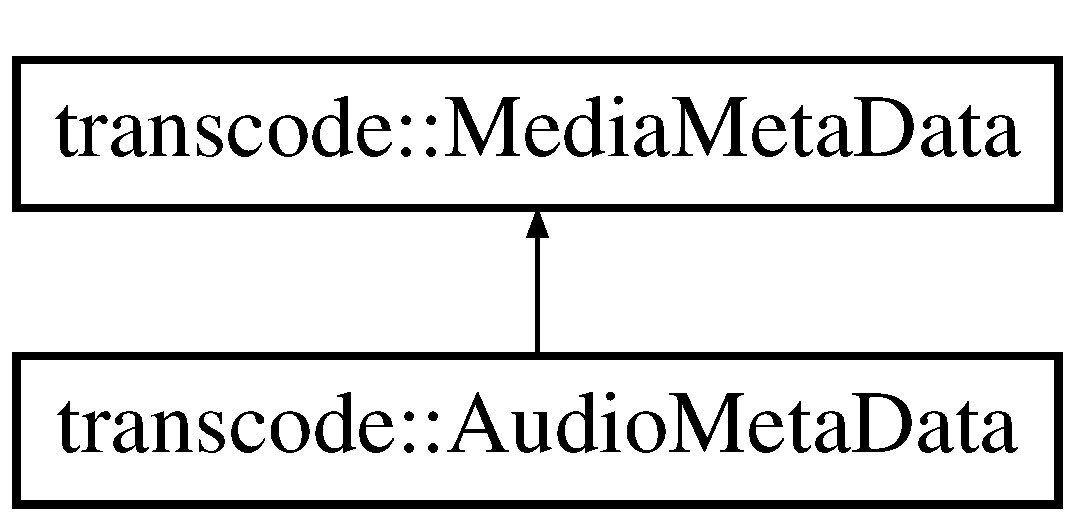
\includegraphics[height=2.000000cm]{structtranscode_1_1AudioMetaData}
\end{center}
\end{figure}
\subsection*{Public Member Functions}
\begin{DoxyCompactItemize}
\item 
\hyperlink{structtranscode_1_1AudioMetaData_ab01057c9c6911c59da09da7de8b43c69}{AudioMetaData} (const std::string \&mimeType, const std::string \&lang, const int \&r, const int \&ch)
\begin{DoxyCompactList}\small\item\em Construct a new AudioDetails struct with the provided mimetype, rate, and channel numbers. \item\end{DoxyCompactList}\end{DoxyCompactItemize}
\subsection*{Public Attributes}
\begin{DoxyCompactItemize}
\item 
\hypertarget{structtranscode_1_1AudioMetaData_a648138cfa52e79c16c1ade849be055c6}{
std::string {\bfseries language}}
\label{structtranscode_1_1AudioMetaData_a648138cfa52e79c16c1ade849be055c6}

\item 
\hypertarget{structtranscode_1_1AudioMetaData_ac4e4d96acd8ee5abf97e63cdc0db46df}{
int {\bfseries rate}}
\label{structtranscode_1_1AudioMetaData_ac4e4d96acd8ee5abf97e63cdc0db46df}

\item 
\hypertarget{structtranscode_1_1AudioMetaData_a1bb969fdca1da86d2cb3f1ec0d490be9}{
int {\bfseries channels}}
\label{structtranscode_1_1AudioMetaData_a1bb969fdca1da86d2cb3f1ec0d490be9}

\end{DoxyCompactItemize}


\subsection{Detailed Description}
Struct to hold all the common attributes for an audio media type. 

Definition at line 63 of file metadata.hpp.



\subsection{Constructor \& Destructor Documentation}
\hypertarget{structtranscode_1_1AudioMetaData_ab01057c9c6911c59da09da7de8b43c69}{
\index{transcode::AudioMetaData@{transcode::AudioMetaData}!AudioMetaData@{AudioMetaData}}
\index{AudioMetaData@{AudioMetaData}!transcode::AudioMetaData@{transcode::AudioMetaData}}
\subsubsection[{AudioMetaData}]{\setlength{\rightskip}{0pt plus 5cm}transcode::AudioMetaData::AudioMetaData (
\begin{DoxyParamCaption}
\item[{const std::string \&}]{mimeType, }
\item[{const std::string \&}]{lang, }
\item[{const int \&}]{r, }
\item[{const int \&}]{ch}
\end{DoxyParamCaption}
)\hspace{0.3cm}{\ttfamily  \mbox{[}inline\mbox{]}}}}
\label{structtranscode_1_1AudioMetaData_ab01057c9c6911c59da09da7de8b43c69}


Construct a new AudioDetails struct with the provided mimetype, rate, and channel numbers. 


\begin{DoxyParams}{Parameters}
{\em mimeType} & -\/ the mimeType for this AudioDetails struct. \\
\hline
{\em lang} & -\/ the language of the stream. \\
\hline
{\em r} & -\/ the sample rate of the data, in samples (per channel) per second. \\
\hline
{\em ch} & -\/ the number of channels of audio data. \\
\hline
\end{DoxyParams}


Definition at line 82 of file metadata.hpp.



The documentation for this struct was generated from the following file:\begin{DoxyCompactItemize}
\item 
src/main/native/metadata.hpp\end{DoxyCompactItemize}

\hypertarget{structtranscode_1_1ContainerMetaData}{
\section{transcode::ContainerMetaData Struct Reference}
\label{structtranscode_1_1ContainerMetaData}\index{transcode::ContainerMetaData@{transcode::ContainerMetaData}}
}


Struct to hold all the common attributes for a container media type.  




{\ttfamily \#include $<$metadata.hpp$>$}

Inheritance diagram for transcode::ContainerMetaData:\begin{figure}[H]
\begin{center}
\leavevmode
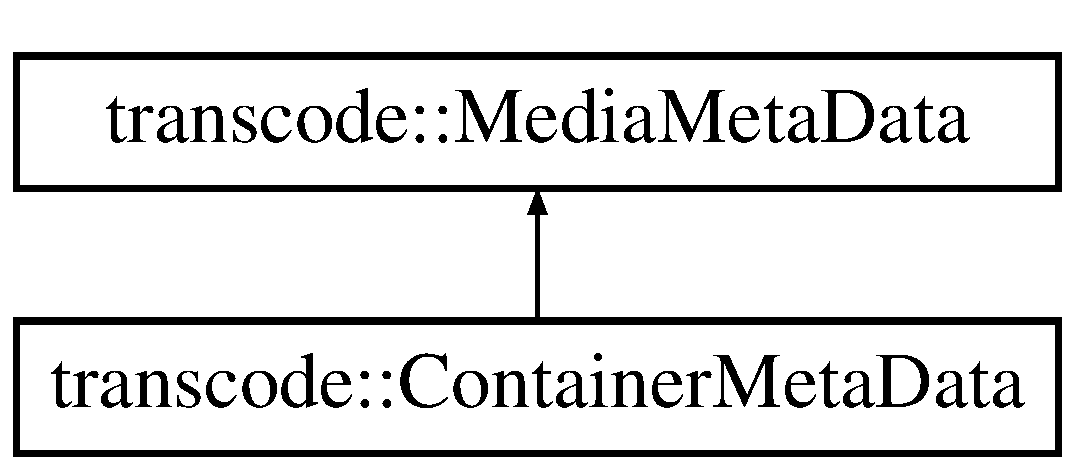
\includegraphics[height=2.000000cm]{structtranscode_1_1ContainerMetaData}
\end{center}
\end{figure}
\subsection*{Public Member Functions}
\begin{DoxyCompactItemize}
\item 
\hyperlink{structtranscode_1_1ContainerMetaData_aaecda8bf6a1ebdaaff17275967b5fb40}{ContainerMetaData} (const std::string \&mimeType, const std::string \&desc, const std::vector$<$ \hyperlink{structtranscode_1_1SubtitleMetaData}{SubtitleMetaData} $>$ \&subDets, const std::vector$<$ \hyperlink{structtranscode_1_1AudioMetaData}{AudioMetaData} $>$ \&audioDets, const std::vector$<$ \hyperlink{structtranscode_1_1VideoMetaData}{VideoMetaData} $>$ \&videoDets)
\begin{DoxyCompactList}\small\item\em Construct a new ContainerDetails struct with the provided mimetype, description, audio, and video details. \item\end{DoxyCompactList}\end{DoxyCompactItemize}
\subsection*{Public Attributes}
\begin{DoxyCompactItemize}
\item 
\hypertarget{structtranscode_1_1ContainerMetaData_a77a95be207cb93b3299b16b22ab37435}{
std::string {\bfseries description}}
\label{structtranscode_1_1ContainerMetaData_a77a95be207cb93b3299b16b22ab37435}

\item 
\hypertarget{structtranscode_1_1ContainerMetaData_abb6c46a666a473437c91383be3cf0a11}{
std::vector$<$ \hyperlink{structtranscode_1_1SubtitleMetaData}{SubtitleMetaData} $>$ {\bfseries subtitleDetails}}
\label{structtranscode_1_1ContainerMetaData_abb6c46a666a473437c91383be3cf0a11}

\item 
\hypertarget{structtranscode_1_1ContainerMetaData_a3c2ee6eac7be55cb351ae3a9ce0d269e}{
std::vector$<$ \hyperlink{structtranscode_1_1AudioMetaData}{AudioMetaData} $>$ {\bfseries audioDetails}}
\label{structtranscode_1_1ContainerMetaData_a3c2ee6eac7be55cb351ae3a9ce0d269e}

\item 
\hypertarget{structtranscode_1_1ContainerMetaData_a301022de11561b8078dd7869be16884e}{
std::vector$<$ \hyperlink{structtranscode_1_1VideoMetaData}{VideoMetaData} $>$ {\bfseries videoDetails}}
\label{structtranscode_1_1ContainerMetaData_a301022de11561b8078dd7869be16884e}

\end{DoxyCompactItemize}


\subsection{Detailed Description}
Struct to hold all the common attributes for a container media type. 

Definition at line 122 of file metadata.hpp.



\subsection{Constructor \& Destructor Documentation}
\hypertarget{structtranscode_1_1ContainerMetaData_aaecda8bf6a1ebdaaff17275967b5fb40}{
\index{transcode::ContainerMetaData@{transcode::ContainerMetaData}!ContainerMetaData@{ContainerMetaData}}
\index{ContainerMetaData@{ContainerMetaData}!transcode::ContainerMetaData@{transcode::ContainerMetaData}}
\subsubsection[{ContainerMetaData}]{\setlength{\rightskip}{0pt plus 5cm}transcode::ContainerMetaData::ContainerMetaData (
\begin{DoxyParamCaption}
\item[{const std::string \&}]{mimeType, }
\item[{const std::string \&}]{desc, }
\item[{const std::vector$<$ {\bf SubtitleMetaData} $>$ \&}]{subDets, }
\item[{const std::vector$<$ {\bf AudioMetaData} $>$ \&}]{audioDets, }
\item[{const std::vector$<$ {\bf VideoMetaData} $>$ \&}]{videoDets}
\end{DoxyParamCaption}
)\hspace{0.3cm}{\ttfamily  \mbox{[}inline\mbox{]}}}}
\label{structtranscode_1_1ContainerMetaData_aaecda8bf6a1ebdaaff17275967b5fb40}


Construct a new ContainerDetails struct with the provided mimetype, description, audio, and video details. 


\begin{DoxyParams}{Parameters}
{\em mimeType} & -\/ the mimeType for this ContainerDetails struct. \\
\hline
{\em desc} & -\/ a description of this container. \\
\hline
{\em subDets} & -\/ a list of subtitle details related to the subtitle streams contained within this container. \\
\hline
{\em audioDets} & -\/ a list of audio details related to the audio streams contained within this container. \\
\hline
{\em videoDets} & -\/ a list of video details related to the video streams contained within this container. \\
\hline
\end{DoxyParams}


Definition at line 150 of file metadata.hpp.



The documentation for this struct was generated from the following file:\begin{DoxyCompactItemize}
\item 
src/main/native/metadata.hpp\end{DoxyCompactItemize}

\hypertarget{classtranscode_1_1util_1_1FFMPEGException}{
\section{transcode::util::FFMPEGException Class Reference}
\label{classtranscode_1_1util_1_1FFMPEGException}\index{transcode::util::FFMPEGException@{transcode::util::FFMPEGException}}
}


Exception that is thrown if something goes wrong with the FFMPEG library.  




{\ttfamily \#include $<$util\_\-ffmpeg.hpp$>$}

Inheritance diagram for transcode::util::FFMPEGException:\begin{figure}[H]
\begin{center}
\leavevmode
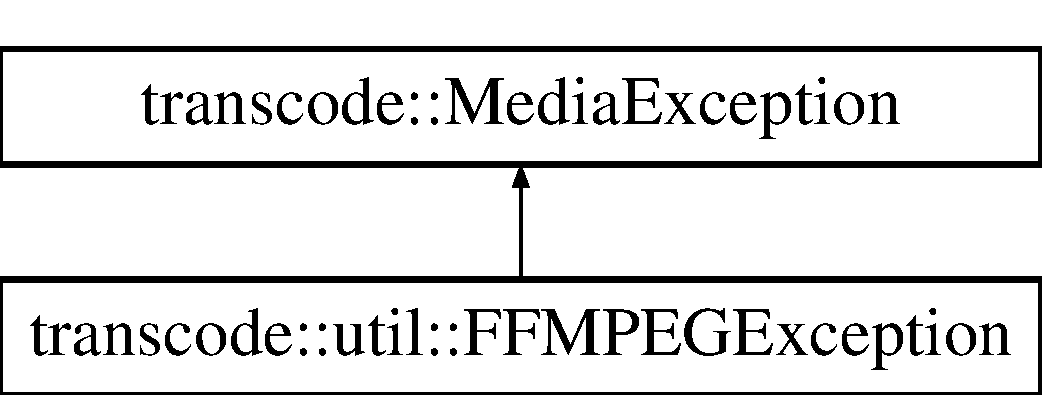
\includegraphics[height=2.000000cm]{classtranscode_1_1util_1_1FFMPEGException}
\end{center}
\end{figure}
\subsection*{Public Member Functions}
\begin{DoxyCompactItemize}
\item 
\hyperlink{classtranscode_1_1util_1_1FFMPEGException_a3e18fe9f063f97e2bcf3780fd957a8ba}{FFMPEGException} ()  throw ()
\begin{DoxyCompactList}\small\item\em Default constructor, set message to empty string and error code to 0. \item\end{DoxyCompactList}\item 
\hyperlink{classtranscode_1_1util_1_1FFMPEGException_ae593dd23fbd854835a78f4adc2c70f90}{FFMPEGException} (const std::string \&msg)  throw ()
\begin{DoxyCompactList}\small\item\em Instantiate a new \hyperlink{classtranscode_1_1util_1_1FFMPEGException}{FFMPEGException} with the provided error message and set the error code to 0. \item\end{DoxyCompactList}\item 
\hyperlink{classtranscode_1_1util_1_1FFMPEGException_a07fe05c4f009f2838f9a9e18ff99e607}{FFMPEGException} (const int \&ec)  throw ()
\begin{DoxyCompactList}\small\item\em Instantiate a new \hyperlink{classtranscode_1_1util_1_1FFMPEGException}{FFMPEGException} with the provided error code and the message set automatically from the error code. \item\end{DoxyCompactList}\item 
\hyperlink{classtranscode_1_1util_1_1FFMPEGException_a0b38fccbe2fdff8d15b50c28a851cdae}{FFMPEGException} (const std::string \&msg, const int \&ec)  throw ()
\begin{DoxyCompactList}\small\item\em Instantiate an \hyperlink{classtranscode_1_1util_1_1FFMPEGException}{FFMPEGException} with the provided message and error code. \item\end{DoxyCompactList}\item 
int \hyperlink{classtranscode_1_1util_1_1FFMPEGException_a08bfd7a8cc1c2dcd5fc54fe700db7806}{getErrorCode} ()
\begin{DoxyCompactList}\small\item\em Get the error code for this exception. \item\end{DoxyCompactList}\end{DoxyCompactItemize}


\subsection{Detailed Description}
Exception that is thrown if something goes wrong with the FFMPEG library. 

Definition at line 60 of file util\_\-ffmpeg.hpp.



\subsection{Constructor \& Destructor Documentation}
\hypertarget{classtranscode_1_1util_1_1FFMPEGException_a3e18fe9f063f97e2bcf3780fd957a8ba}{
\index{transcode::util::FFMPEGException@{transcode::util::FFMPEGException}!FFMPEGException@{FFMPEGException}}
\index{FFMPEGException@{FFMPEGException}!transcode::util::FFMPEGException@{transcode::util::FFMPEGException}}
\subsubsection[{FFMPEGException}]{\setlength{\rightskip}{0pt plus 5cm}transcode::util::FFMPEGException::FFMPEGException (
\begin{DoxyParamCaption}
{}
\end{DoxyParamCaption}
)  throw ()\hspace{0.3cm}{\ttfamily  \mbox{[}inline\mbox{]}}}}
\label{classtranscode_1_1util_1_1FFMPEGException_a3e18fe9f063f97e2bcf3780fd957a8ba}


Default constructor, set message to empty string and error code to 0. 



Definition at line 69 of file util\_\-ffmpeg.hpp.

\hypertarget{classtranscode_1_1util_1_1FFMPEGException_ae593dd23fbd854835a78f4adc2c70f90}{
\index{transcode::util::FFMPEGException@{transcode::util::FFMPEGException}!FFMPEGException@{FFMPEGException}}
\index{FFMPEGException@{FFMPEGException}!transcode::util::FFMPEGException@{transcode::util::FFMPEGException}}
\subsubsection[{FFMPEGException}]{\setlength{\rightskip}{0pt plus 5cm}transcode::util::FFMPEGException::FFMPEGException (
\begin{DoxyParamCaption}
\item[{const std::string \&}]{msg}
\end{DoxyParamCaption}
)  throw ()\hspace{0.3cm}{\ttfamily  \mbox{[}inline\mbox{]}}}}
\label{classtranscode_1_1util_1_1FFMPEGException_ae593dd23fbd854835a78f4adc2c70f90}


Instantiate a new \hyperlink{classtranscode_1_1util_1_1FFMPEGException}{FFMPEGException} with the provided error message and set the error code to 0. 


\begin{DoxyParams}{Parameters}
{\em msg} & -\/ the message for this exception. \\
\hline
\end{DoxyParams}


Definition at line 79 of file util\_\-ffmpeg.hpp.

\hypertarget{classtranscode_1_1util_1_1FFMPEGException_a07fe05c4f009f2838f9a9e18ff99e607}{
\index{transcode::util::FFMPEGException@{transcode::util::FFMPEGException}!FFMPEGException@{FFMPEGException}}
\index{FFMPEGException@{FFMPEGException}!transcode::util::FFMPEGException@{transcode::util::FFMPEGException}}
\subsubsection[{FFMPEGException}]{\setlength{\rightskip}{0pt plus 5cm}transcode::util::FFMPEGException::FFMPEGException (
\begin{DoxyParamCaption}
\item[{const int \&}]{ec}
\end{DoxyParamCaption}
)  throw ()\hspace{0.3cm}{\ttfamily  \mbox{[}inline\mbox{]}}}}
\label{classtranscode_1_1util_1_1FFMPEGException_a07fe05c4f009f2838f9a9e18ff99e607}


Instantiate a new \hyperlink{classtranscode_1_1util_1_1FFMPEGException}{FFMPEGException} with the provided error code and the message set automatically from the error code. 


\begin{DoxyParams}{Parameters}
{\em ec} & -\/ the FFMPEG error code for this exception. \\
\hline
\end{DoxyParams}


Definition at line 89 of file util\_\-ffmpeg.hpp.

\hypertarget{classtranscode_1_1util_1_1FFMPEGException_a0b38fccbe2fdff8d15b50c28a851cdae}{
\index{transcode::util::FFMPEGException@{transcode::util::FFMPEGException}!FFMPEGException@{FFMPEGException}}
\index{FFMPEGException@{FFMPEGException}!transcode::util::FFMPEGException@{transcode::util::FFMPEGException}}
\subsubsection[{FFMPEGException}]{\setlength{\rightskip}{0pt plus 5cm}transcode::util::FFMPEGException::FFMPEGException (
\begin{DoxyParamCaption}
\item[{const std::string \&}]{msg, }
\item[{const int \&}]{ec}
\end{DoxyParamCaption}
)  throw ()\hspace{0.3cm}{\ttfamily  \mbox{[}inline\mbox{]}}}}
\label{classtranscode_1_1util_1_1FFMPEGException_a0b38fccbe2fdff8d15b50c28a851cdae}


Instantiate an \hyperlink{classtranscode_1_1util_1_1FFMPEGException}{FFMPEGException} with the provided message and error code. 


\begin{DoxyParams}{Parameters}
{\em msg} & -\/ the message for this exception. \\
\hline
{\em ec} & -\/ the FFMPEG error code for this exception. \\
\hline
\end{DoxyParams}


Definition at line 99 of file util\_\-ffmpeg.hpp.



\subsection{Member Function Documentation}
\hypertarget{classtranscode_1_1util_1_1FFMPEGException_a08bfd7a8cc1c2dcd5fc54fe700db7806}{
\index{transcode::util::FFMPEGException@{transcode::util::FFMPEGException}!getErrorCode@{getErrorCode}}
\index{getErrorCode@{getErrorCode}!transcode::util::FFMPEGException@{transcode::util::FFMPEGException}}
\subsubsection[{getErrorCode}]{\setlength{\rightskip}{0pt plus 5cm}int transcode::util::FFMPEGException::getErrorCode (
\begin{DoxyParamCaption}
{}
\end{DoxyParamCaption}
)\hspace{0.3cm}{\ttfamily  \mbox{[}inline\mbox{]}}}}
\label{classtranscode_1_1util_1_1FFMPEGException_a08bfd7a8cc1c2dcd5fc54fe700db7806}


Get the error code for this exception. 

\begin{DoxyReturn}{Returns}
the error code for this exception. 
\end{DoxyReturn}


Definition at line 111 of file util\_\-ffmpeg.hpp.



The documentation for this class was generated from the following file:\begin{DoxyCompactItemize}
\item 
src/main/native/util/\hyperlink{util__ffmpeg_8hpp}{util\_\-ffmpeg.hpp}\end{DoxyCompactItemize}

\hypertarget{classtranscode_1_1util_1_1FfmpegSingleton}{
\section{transcode::util::FfmpegSingleton Class Reference}
\label{classtranscode_1_1util_1_1FfmpegSingleton}\index{transcode::util::FfmpegSingleton@{transcode::util::FfmpegSingleton}}
}


A singleton class that provides all the implementations for the FFMPEG functions.  


\subsection*{Public Member Functions}
\begin{DoxyCompactItemize}
\item 
\hypertarget{classtranscode_1_1util_1_1FfmpegSingleton_afcaff88a65a5a7392ef221c6124c7f47}{
std::string {\bfseries ffmpegErrorMessage} (int errorCode) const }
\label{classtranscode_1_1util_1_1FfmpegSingleton_afcaff88a65a5a7392ef221c6124c7f47}

\item 
\hypertarget{classtranscode_1_1util_1_1FfmpegSingleton_a2df8734a7a6b106757b1c9041ed0b3e8}{
AVFormatContext $\ast$ {\bfseries retrieveAVFormatContext} (const std::string \&filePath) const }
\label{classtranscode_1_1util_1_1FfmpegSingleton_a2df8734a7a6b106757b1c9041ed0b3e8}

\item 
\hypertarget{classtranscode_1_1util_1_1FfmpegSingleton_a82ca88208ef34718ee20ee99beb25101}{
std::vector$<$ \hyperlink{structtranscode_1_1SubtitleMetaData}{SubtitleMetaData} $>$ {\bfseries extractSubtitleDetails} (const AVFormatContext $\ast$videoFile) const }
\label{classtranscode_1_1util_1_1FfmpegSingleton_a82ca88208ef34718ee20ee99beb25101}

\item 
\hypertarget{classtranscode_1_1util_1_1FfmpegSingleton_aac69472179a03040d17d072c1987c5ce}{
std::vector$<$ \hyperlink{structtranscode_1_1AudioMetaData}{AudioMetaData} $>$ {\bfseries extractAudioDetails} (const AVFormatContext $\ast$videoFile) const }
\label{classtranscode_1_1util_1_1FfmpegSingleton_aac69472179a03040d17d072c1987c5ce}

\item 
\hypertarget{classtranscode_1_1util_1_1FfmpegSingleton_a7ecd105f56b9ac9e1c619453f4c872f2}{
std::vector$<$ \hyperlink{structtranscode_1_1VideoMetaData}{VideoMetaData} $>$ {\bfseries extractVideoDetails} (const AVFormatContext $\ast$videoFile) const }
\label{classtranscode_1_1util_1_1FfmpegSingleton_a7ecd105f56b9ac9e1c619453f4c872f2}

\item 
\hypertarget{classtranscode_1_1util_1_1FfmpegSingleton_a41251296d417f2751754b5d7f7f6205a}{
\hyperlink{structtranscode_1_1ContainerMetaData}{ContainerMetaData} {\bfseries buildContainerDetail} (const AVFormatContext $\ast$videoFile) const }
\label{classtranscode_1_1util_1_1FfmpegSingleton_a41251296d417f2751754b5d7f7f6205a}

\item 
\hypertarget{classtranscode_1_1util_1_1FfmpegSingleton_a9e30a10b3a4b443dfec543da746bab6e}{
void {\bfseries closeCodecs} (AVFormatContext $\ast$videoFile) const   throw (FFMPEGException)}
\label{classtranscode_1_1util_1_1FfmpegSingleton_a9e30a10b3a4b443dfec543da746bab6e}

\end{DoxyCompactItemize}
\subsection*{Static Public Member Functions}
\begin{DoxyCompactItemize}
\item 
\hypertarget{classtranscode_1_1util_1_1FfmpegSingleton_a37162eb4957bbfec135c6e24857363eb}{
static const \hyperlink{classtranscode_1_1util_1_1FfmpegSingleton}{FfmpegSingleton} \& {\bfseries getInstance} ()}
\label{classtranscode_1_1util_1_1FfmpegSingleton_a37162eb4957bbfec135c6e24857363eb}

\end{DoxyCompactItemize}


\subsection{Detailed Description}
A singleton class that provides all the implementations for the FFMPEG functions. This class has been created because FFMPEG requires initialisation, so if all function calls are invoked through this singleton it is guaranteed that the initialisation has been carried out and will only ever be carried out once.

The structure of this singleton was taken from here: \href{http://stackoverflow.com/questions/1008019/c-singleton-design-pattern}{\tt http://stackoverflow.com/questions/1008019/c-\/singleton-\/design-\/pattern} 

Definition at line 268 of file util\_\-ffmpeg.cpp.



The documentation for this class was generated from the following file:\begin{DoxyCompactItemize}
\item 
src/main/native/util/\hyperlink{util__ffmpeg_8cpp}{util\_\-ffmpeg.cpp}\end{DoxyCompactItemize}

\hypertarget{classtranscode_1_1util_1_1File}{
\section{transcode::util::File Class Reference}
\label{classtranscode_1_1util_1_1File}\index{transcode::util::File@{transcode::util::File}}
}


A class that represents a file on the file system, it can be used to access meta data about the file.  




{\ttfamily \#include $<$util\_\-file.hpp$>$}

\subsection*{Public Member Functions}
\begin{DoxyCompactItemize}
\item 
\hyperlink{classtranscode_1_1util_1_1File_ad459dd3cc090abbbb220a87f1909d7f9}{File} ()
\begin{DoxyCompactList}\small\item\em Instantiate an empty \hyperlink{classtranscode_1_1util_1_1File}{File} object. \item\end{DoxyCompactList}\item 
\hyperlink{classtranscode_1_1util_1_1File_a60d3a3b965968122d87e319c8181c866}{File} (std::string path)  throw (FileException)
\begin{DoxyCompactList}\small\item\em Instantiate a new \hyperlink{classtranscode_1_1util_1_1File}{File} object that will be populated from the meta data of the file at the provided path. \item\end{DoxyCompactList}\item 
std::string \hyperlink{classtranscode_1_1util_1_1File_a80cc652ec8b51ecac79dfcf469ae3c2f}{getName} () const 
\begin{DoxyCompactList}\small\item\em Get the name of the related file minus the path. \item\end{DoxyCompactList}\item 
std::string \hyperlink{classtranscode_1_1util_1_1File_a22b68c8fa9d48982164da648c18c4f09}{getPath} () const 
\begin{DoxyCompactList}\small\item\em Get the full path of the file that was used to create this object. \item\end{DoxyCompactList}\item 
std::string \hyperlink{classtranscode_1_1util_1_1File_a839681fa33d88cd41aeedef33eccef35}{getAbsolutePath} () const 
\begin{DoxyCompactList}\small\item\em Get the absolute path of the file. \item\end{DoxyCompactList}\item 
std::string \hyperlink{classtranscode_1_1util_1_1File_ab5f643ce545eed3914dbb7507211235b}{getRelativePath} () const 
\begin{DoxyCompactList}\small\item\em Get the relative path of the file to the current running directory. \item\end{DoxyCompactList}\item 
unsigned long \hyperlink{classtranscode_1_1util_1_1File_aaf1d1302f91e67f5953fa2964c2dd8af}{getSize} () const 
\begin{DoxyCompactList}\small\item\em Get the size of the related file in bytes. \item\end{DoxyCompactList}\end{DoxyCompactItemize}


\subsection{Detailed Description}
A class that represents a file on the file system, it can be used to access meta data about the file. 

Definition at line 66 of file util\_\-file.hpp.



\subsection{Constructor \& Destructor Documentation}
\hypertarget{classtranscode_1_1util_1_1File_ad459dd3cc090abbbb220a87f1909d7f9}{
\index{transcode::util::File@{transcode::util::File}!File@{File}}
\index{File@{File}!transcode::util::File@{transcode::util::File}}
\subsubsection[{File}]{\setlength{\rightskip}{0pt plus 5cm}transcode::util::File::File (
\begin{DoxyParamCaption}
{}
\end{DoxyParamCaption}
)\hspace{0.3cm}{\ttfamily  \mbox{[}inline\mbox{]}}}}
\label{classtranscode_1_1util_1_1File_ad459dd3cc090abbbb220a87f1909d7f9}


Instantiate an empty \hyperlink{classtranscode_1_1util_1_1File}{File} object. 



Definition at line 80 of file util\_\-file.hpp.

\hypertarget{classtranscode_1_1util_1_1File_a60d3a3b965968122d87e319c8181c866}{
\index{transcode::util::File@{transcode::util::File}!File@{File}}
\index{File@{File}!transcode::util::File@{transcode::util::File}}
\subsubsection[{File}]{\setlength{\rightskip}{0pt plus 5cm}transcode::util::File::File (
\begin{DoxyParamCaption}
\item[{std::string}]{path}
\end{DoxyParamCaption}
)  throw ({\bf FileException})}}
\label{classtranscode_1_1util_1_1File_a60d3a3b965968122d87e319c8181c866}


Instantiate a new \hyperlink{classtranscode_1_1util_1_1File}{File} object that will be populated from the meta data of the file at the provided path. 


\begin{DoxyParams}{Parameters}
{\em path} & -\/ the path to the file that will be inspected. \\
\hline
\end{DoxyParams}


Definition at line 34 of file util\_\-file.cpp.



\subsection{Member Function Documentation}
\hypertarget{classtranscode_1_1util_1_1File_a839681fa33d88cd41aeedef33eccef35}{
\index{transcode::util::File@{transcode::util::File}!getAbsolutePath@{getAbsolutePath}}
\index{getAbsolutePath@{getAbsolutePath}!transcode::util::File@{transcode::util::File}}
\subsubsection[{getAbsolutePath}]{\setlength{\rightskip}{0pt plus 5cm}std::string transcode::util::File::getAbsolutePath (
\begin{DoxyParamCaption}
{}
\end{DoxyParamCaption}
) const\hspace{0.3cm}{\ttfamily  \mbox{[}inline\mbox{]}}}}
\label{classtranscode_1_1util_1_1File_a839681fa33d88cd41aeedef33eccef35}


Get the absolute path of the file. 

\begin{DoxyReturn}{Returns}
the absolute path of the file. 
\end{DoxyReturn}


Definition at line 121 of file util\_\-file.hpp.

\hypertarget{classtranscode_1_1util_1_1File_a80cc652ec8b51ecac79dfcf469ae3c2f}{
\index{transcode::util::File@{transcode::util::File}!getName@{getName}}
\index{getName@{getName}!transcode::util::File@{transcode::util::File}}
\subsubsection[{getName}]{\setlength{\rightskip}{0pt plus 5cm}std::string transcode::util::File::getName (
\begin{DoxyParamCaption}
{}
\end{DoxyParamCaption}
) const\hspace{0.3cm}{\ttfamily  \mbox{[}inline\mbox{]}}}}
\label{classtranscode_1_1util_1_1File_a80cc652ec8b51ecac79dfcf469ae3c2f}


Get the name of the related file minus the path. 

\begin{DoxyReturn}{Returns}
the name of the file. 
\end{DoxyReturn}


Definition at line 101 of file util\_\-file.hpp.

\hypertarget{classtranscode_1_1util_1_1File_a22b68c8fa9d48982164da648c18c4f09}{
\index{transcode::util::File@{transcode::util::File}!getPath@{getPath}}
\index{getPath@{getPath}!transcode::util::File@{transcode::util::File}}
\subsubsection[{getPath}]{\setlength{\rightskip}{0pt plus 5cm}std::string transcode::util::File::getPath (
\begin{DoxyParamCaption}
{}
\end{DoxyParamCaption}
) const\hspace{0.3cm}{\ttfamily  \mbox{[}inline\mbox{]}}}}
\label{classtranscode_1_1util_1_1File_a22b68c8fa9d48982164da648c18c4f09}


Get the full path of the file that was used to create this object. 

\begin{DoxyReturn}{Returns}
the path of the file. 
\end{DoxyReturn}


Definition at line 111 of file util\_\-file.hpp.

\hypertarget{classtranscode_1_1util_1_1File_ab5f643ce545eed3914dbb7507211235b}{
\index{transcode::util::File@{transcode::util::File}!getRelativePath@{getRelativePath}}
\index{getRelativePath@{getRelativePath}!transcode::util::File@{transcode::util::File}}
\subsubsection[{getRelativePath}]{\setlength{\rightskip}{0pt plus 5cm}std::string transcode::util::File::getRelativePath (
\begin{DoxyParamCaption}
{}
\end{DoxyParamCaption}
) const\hspace{0.3cm}{\ttfamily  \mbox{[}inline\mbox{]}}}}
\label{classtranscode_1_1util_1_1File_ab5f643ce545eed3914dbb7507211235b}


Get the relative path of the file to the current running directory. 

\begin{DoxyReturn}{Returns}
the relative path of the file. 
\end{DoxyReturn}


Definition at line 131 of file util\_\-file.hpp.

\hypertarget{classtranscode_1_1util_1_1File_aaf1d1302f91e67f5953fa2964c2dd8af}{
\index{transcode::util::File@{transcode::util::File}!getSize@{getSize}}
\index{getSize@{getSize}!transcode::util::File@{transcode::util::File}}
\subsubsection[{getSize}]{\setlength{\rightskip}{0pt plus 5cm}unsigned long transcode::util::File::getSize (
\begin{DoxyParamCaption}
{}
\end{DoxyParamCaption}
) const\hspace{0.3cm}{\ttfamily  \mbox{[}inline\mbox{]}}}}
\label{classtranscode_1_1util_1_1File_aaf1d1302f91e67f5953fa2964c2dd8af}


Get the size of the related file in bytes. 

\begin{DoxyReturn}{Returns}
the size of the file. 
\end{DoxyReturn}


Definition at line 141 of file util\_\-file.hpp.



The documentation for this class was generated from the following files:\begin{DoxyCompactItemize}
\item 
src/main/native/util/\hyperlink{util__file_8hpp}{util\_\-file.hpp}\item 
src/main/native/util/\hyperlink{util__file_8cpp}{util\_\-file.cpp}\end{DoxyCompactItemize}

\hypertarget{classtranscode_1_1util_1_1FileException}{
\section{transcode::util::FileException Class Reference}
\label{classtranscode_1_1util_1_1FileException}\index{transcode::util::FileException@{transcode::util::FileException}}
}


Inherits std::exception.

\subsection*{Public Member Functions}
\begin{DoxyCompactItemize}
\item 
\hyperlink{classtranscode_1_1util_1_1FileException_a5b20347ec159197cb226aecca43096d2}{FileException} ()  throw ()
\begin{DoxyCompactList}\small\item\em Default constructor, set the message to empty string. \item\end{DoxyCompactList}\item 
\hyperlink{classtranscode_1_1util_1_1FileException_a49d8ab6a50387dbe1a3e82f22c0f6450}{FileException} (std::string message)  throw ()
\begin{DoxyCompactList}\small\item\em Instantiate a \hyperlink{classtranscode_1_1util_1_1FileException}{FileException} object with the provided message. \item\end{DoxyCompactList}\item 
\hypertarget{classtranscode_1_1util_1_1FileException_aebbce570a698c3909fdd614bea311f49}{
const char $\ast$ {\bfseries what} () const   throw ()}
\label{classtranscode_1_1util_1_1FileException_aebbce570a698c3909fdd614bea311f49}

\end{DoxyCompactItemize}


\subsection{Detailed Description}


Definition at line 34 of file util\_\-file.hpp.



\subsection{Constructor \& Destructor Documentation}
\hypertarget{classtranscode_1_1util_1_1FileException_a5b20347ec159197cb226aecca43096d2}{
\index{transcode::util::FileException@{transcode::util::FileException}!FileException@{FileException}}
\index{FileException@{FileException}!transcode::util::FileException@{transcode::util::FileException}}
\subsubsection[{FileException}]{\setlength{\rightskip}{0pt plus 5cm}transcode::util::FileException::FileException (
\begin{DoxyParamCaption}
{}
\end{DoxyParamCaption}
)  throw ()\hspace{0.3cm}{\ttfamily  \mbox{[}inline\mbox{]}}}}
\label{classtranscode_1_1util_1_1FileException_a5b20347ec159197cb226aecca43096d2}


Default constructor, set the message to empty string. 



Definition at line 43 of file util\_\-file.hpp.

\hypertarget{classtranscode_1_1util_1_1FileException_a49d8ab6a50387dbe1a3e82f22c0f6450}{
\index{transcode::util::FileException@{transcode::util::FileException}!FileException@{FileException}}
\index{FileException@{FileException}!transcode::util::FileException@{transcode::util::FileException}}
\subsubsection[{FileException}]{\setlength{\rightskip}{0pt plus 5cm}transcode::util::FileException::FileException (
\begin{DoxyParamCaption}
\item[{std::string}]{message}
\end{DoxyParamCaption}
)  throw ()\hspace{0.3cm}{\ttfamily  \mbox{[}inline\mbox{]}}}}
\label{classtranscode_1_1util_1_1FileException_a49d8ab6a50387dbe1a3e82f22c0f6450}


Instantiate a \hyperlink{classtranscode_1_1util_1_1FileException}{FileException} object with the provided message. 



Definition at line 50 of file util\_\-file.hpp.



The documentation for this class was generated from the following file:\begin{DoxyCompactItemize}
\item 
src/main/native/util/\hyperlink{util__file_8hpp}{util\_\-file.hpp}\end{DoxyCompactItemize}

\hypertarget{classtranscode_1_1MediaException}{
\section{transcode::MediaException Class Reference}
\label{classtranscode_1_1MediaException}\index{transcode::MediaException@{transcode::MediaException}}
}


An exception that is thrown if something goes wrong during media processing.  




{\ttfamily \#include $<$error.hpp$>$}

Inheritance diagram for transcode::MediaException:\begin{figure}[H]
\begin{center}
\leavevmode
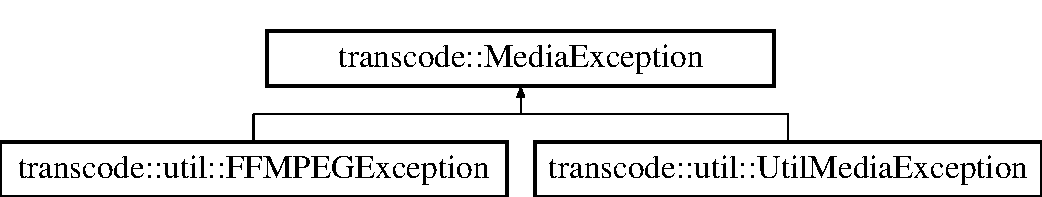
\includegraphics[height=2.000000cm]{classtranscode_1_1MediaException}
\end{center}
\end{figure}
\subsection*{Public Member Functions}
\begin{DoxyCompactItemize}
\item 
\hyperlink{classtranscode_1_1MediaException_ab7bb21af19aaa3d36e45a4504b538922}{MediaException} ()  throw ()
\begin{DoxyCompactList}\small\item\em Instantiate an empty \hyperlink{classtranscode_1_1MediaException}{MediaException} object. \item\end{DoxyCompactList}\item 
\hyperlink{classtranscode_1_1MediaException_ab18693f11e51b0c9684e5c6df0901313}{MediaException} (std::string message)  throw ()
\begin{DoxyCompactList}\small\item\em Instantiate a \hyperlink{classtranscode_1_1MediaException}{MediaException} object with the provided message. \item\end{DoxyCompactList}\item 
\hypertarget{classtranscode_1_1MediaException_ab662d6628667f2105adf95744f23d357}{
const char $\ast$ {\bfseries what} () const   throw ()}
\label{classtranscode_1_1MediaException_ab662d6628667f2105adf95744f23d357}

\end{DoxyCompactItemize}


\subsection{Detailed Description}
An exception that is thrown if something goes wrong during media processing. 

Definition at line 20 of file error.hpp.



\subsection{Constructor \& Destructor Documentation}
\hypertarget{classtranscode_1_1MediaException_ab7bb21af19aaa3d36e45a4504b538922}{
\index{transcode::MediaException@{transcode::MediaException}!MediaException@{MediaException}}
\index{MediaException@{MediaException}!transcode::MediaException@{transcode::MediaException}}
\subsubsection[{MediaException}]{\setlength{\rightskip}{0pt plus 5cm}transcode::MediaException::MediaException (
\begin{DoxyParamCaption}
{}
\end{DoxyParamCaption}
)  throw ()\hspace{0.3cm}{\ttfamily  \mbox{[}inline\mbox{]}}}}
\label{classtranscode_1_1MediaException_ab7bb21af19aaa3d36e45a4504b538922}


Instantiate an empty \hyperlink{classtranscode_1_1MediaException}{MediaException} object. 



Definition at line 29 of file error.hpp.

\hypertarget{classtranscode_1_1MediaException_ab18693f11e51b0c9684e5c6df0901313}{
\index{transcode::MediaException@{transcode::MediaException}!MediaException@{MediaException}}
\index{MediaException@{MediaException}!transcode::MediaException@{transcode::MediaException}}
\subsubsection[{MediaException}]{\setlength{\rightskip}{0pt plus 5cm}transcode::MediaException::MediaException (
\begin{DoxyParamCaption}
\item[{std::string}]{message}
\end{DoxyParamCaption}
)  throw ()\hspace{0.3cm}{\ttfamily  \mbox{[}inline\mbox{]}}}}
\label{classtranscode_1_1MediaException_ab18693f11e51b0c9684e5c6df0901313}


Instantiate a \hyperlink{classtranscode_1_1MediaException}{MediaException} object with the provided message. 


\begin{DoxyParams}{Parameters}
{\em message} & -\/ the message for the new exception. \\
\hline
\end{DoxyParams}


Definition at line 38 of file error.hpp.



The documentation for this class was generated from the following file:\begin{DoxyCompactItemize}
\item 
src/main/native/error.hpp\end{DoxyCompactItemize}

\hypertarget{structtranscode_1_1MediaFileMetaData}{
\section{transcode::MediaFileMetaData Struct Reference}
\label{structtranscode_1_1MediaFileMetaData}\index{transcode::MediaFileMetaData@{transcode::MediaFileMetaData}}
}


Struct to hold all the common attributes for a media file.  




{\ttfamily \#include $<$metadata.hpp$>$}

\subsection*{Public Member Functions}
\begin{DoxyCompactItemize}
\item 
\hyperlink{structtranscode_1_1MediaFileMetaData_a23221e0853537b4be8280ce2b75b621c}{MediaFileMetaData} (const \hyperlink{structtranscode_1_1ContainerMetaData}{ContainerMetaData} \&cont, const std::string \&p, const std::string \&n, const int \&s)
\begin{DoxyCompactList}\small\item\em Construct a new MediaFileDetail struct with the provided container, path, name, and size. \item\end{DoxyCompactList}\end{DoxyCompactItemize}
\subsection*{Public Attributes}
\begin{DoxyCompactItemize}
\item 
\hypertarget{structtranscode_1_1MediaFileMetaData_a2f713e86bd7ee716c59ef0701930e795}{
\hyperlink{structtranscode_1_1ContainerMetaData}{ContainerMetaData} {\bfseries container}}
\label{structtranscode_1_1MediaFileMetaData_a2f713e86bd7ee716c59ef0701930e795}

\item 
\hypertarget{structtranscode_1_1MediaFileMetaData_a9159286b1d2e7f014d64679088d60d8f}{
std::string {\bfseries path}}
\label{structtranscode_1_1MediaFileMetaData_a9159286b1d2e7f014d64679088d60d8f}

\item 
\hypertarget{structtranscode_1_1MediaFileMetaData_a0102c41b4de772f5c5b0ad0492d33e6d}{
std::string {\bfseries name}}
\label{structtranscode_1_1MediaFileMetaData_a0102c41b4de772f5c5b0ad0492d33e6d}

\item 
\hypertarget{structtranscode_1_1MediaFileMetaData_a52d9764c013a59a8e1c505634af82706}{
int {\bfseries size}}
\label{structtranscode_1_1MediaFileMetaData_a52d9764c013a59a8e1c505634af82706}

\end{DoxyCompactItemize}


\subsection{Detailed Description}
Struct to hold all the common attributes for a media file. 

Definition at line 166 of file metadata.hpp.



\subsection{Constructor \& Destructor Documentation}
\hypertarget{structtranscode_1_1MediaFileMetaData_a23221e0853537b4be8280ce2b75b621c}{
\index{transcode::MediaFileMetaData@{transcode::MediaFileMetaData}!MediaFileMetaData@{MediaFileMetaData}}
\index{MediaFileMetaData@{MediaFileMetaData}!transcode::MediaFileMetaData@{transcode::MediaFileMetaData}}
\subsubsection[{MediaFileMetaData}]{\setlength{\rightskip}{0pt plus 5cm}transcode::MediaFileMetaData::MediaFileMetaData (
\begin{DoxyParamCaption}
\item[{const {\bf ContainerMetaData} \&}]{cont, }
\item[{const std::string \&}]{p, }
\item[{const std::string \&}]{n, }
\item[{const int \&}]{s}
\end{DoxyParamCaption}
)\hspace{0.3cm}{\ttfamily  \mbox{[}inline\mbox{]}}}}
\label{structtranscode_1_1MediaFileMetaData_a23221e0853537b4be8280ce2b75b621c}


Construct a new MediaFileDetail struct with the provided container, path, name, and size. 


\begin{DoxyParams}{Parameters}
{\em cont} & -\/ the container of this media file. \\
\hline
{\em p} & -\/ a full path of this media file. \\
\hline
{\em n} & -\/ the name of this media file minus the path. \\
\hline
{\em s} & -\/ the size of this media file in bytes. \\
\hline
\end{DoxyParams}


Definition at line 186 of file metadata.hpp.



The documentation for this struct was generated from the following file:\begin{DoxyCompactItemize}
\item 
src/main/native/metadata.hpp\end{DoxyCompactItemize}

\hypertarget{structtranscode_1_1MediaMetaData}{
\section{transcode::MediaMetaData Struct Reference}
\label{structtranscode_1_1MediaMetaData}\index{transcode::MediaMetaData@{transcode::MediaMetaData}}
}


Struct to hold all the common attributes for a media type.  




{\ttfamily \#include $<$metadata.hpp$>$}

Inheritance diagram for transcode::MediaMetaData:\begin{figure}[H]
\begin{center}
\leavevmode
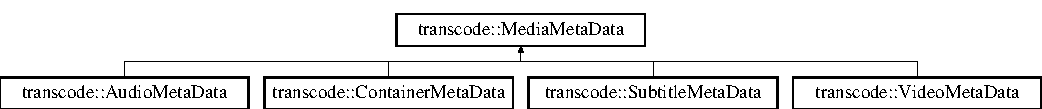
\includegraphics[height=1.465969cm]{structtranscode_1_1MediaMetaData}
\end{center}
\end{figure}
\subsection*{Public Member Functions}
\begin{DoxyCompactItemize}
\item 
\hyperlink{structtranscode_1_1MediaMetaData_ab9e99a1ca5a89900e6514ae29b40f1e6}{MediaMetaData} (const std::string \&mType)
\begin{DoxyCompactList}\small\item\em Construct a new \hyperlink{structtranscode_1_1MediaMetaData}{MediaMetaData} struct with the provided mimetype. \item\end{DoxyCompactList}\end{DoxyCompactItemize}
\subsection*{Public Attributes}
\begin{DoxyCompactItemize}
\item 
\hypertarget{structtranscode_1_1MediaMetaData_a83154da5545a20f2bb9f36a5406e01a1}{
std::string {\bfseries mimeType}}
\label{structtranscode_1_1MediaMetaData_a83154da5545a20f2bb9f36a5406e01a1}

\end{DoxyCompactItemize}


\subsection{Detailed Description}
Struct to hold all the common attributes for a media type. 

Definition at line 19 of file metadata.hpp.



\subsection{Constructor \& Destructor Documentation}
\hypertarget{structtranscode_1_1MediaMetaData_ab9e99a1ca5a89900e6514ae29b40f1e6}{
\index{transcode::MediaMetaData@{transcode::MediaMetaData}!MediaMetaData@{MediaMetaData}}
\index{MediaMetaData@{MediaMetaData}!transcode::MediaMetaData@{transcode::MediaMetaData}}
\subsubsection[{MediaMetaData}]{\setlength{\rightskip}{0pt plus 5cm}transcode::MediaMetaData::MediaMetaData (
\begin{DoxyParamCaption}
\item[{const std::string \&}]{mType}
\end{DoxyParamCaption}
)\hspace{0.3cm}{\ttfamily  \mbox{[}inline\mbox{]}}}}
\label{structtranscode_1_1MediaMetaData_ab9e99a1ca5a89900e6514ae29b40f1e6}


Construct a new \hyperlink{structtranscode_1_1MediaMetaData}{MediaMetaData} struct with the provided mimetype. 


\begin{DoxyParams}{Parameters}
{\em mType} & -\/ the mimeType for this MediaType struct. \\
\hline
\end{DoxyParams}


Definition at line 32 of file metadata.hpp.



The documentation for this struct was generated from the following file:\begin{DoxyCompactItemize}
\item 
src/main/native/metadata.hpp\end{DoxyCompactItemize}

\hypertarget{structtranscode_1_1SubtitleMetaData}{
\section{transcode::SubtitleMetaData Struct Reference}
\label{structtranscode_1_1SubtitleMetaData}\index{transcode::SubtitleMetaData@{transcode::SubtitleMetaData}}
}


Struct to hold all the common attributes for a subtitle media type.  




{\ttfamily \#include $<$metadata.hpp$>$}

Inheritance diagram for transcode::SubtitleMetaData:\begin{figure}[H]
\begin{center}
\leavevmode
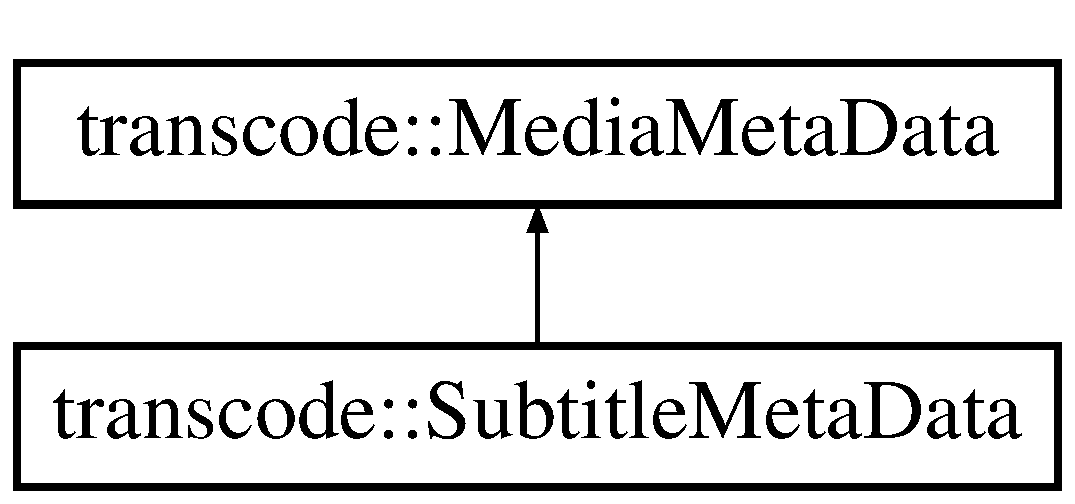
\includegraphics[height=2.000000cm]{structtranscode_1_1SubtitleMetaData}
\end{center}
\end{figure}
\subsection*{Public Member Functions}
\begin{DoxyCompactItemize}
\item 
\hyperlink{structtranscode_1_1SubtitleMetaData_a28480e38e52a8a2bf854399cbe06319c}{SubtitleMetaData} (const std::string \&mimeType, const std::string \&lang)
\begin{DoxyCompactList}\small\item\em Construct a new SubtitleDetail struct with the provided mimetype and language. \item\end{DoxyCompactList}\end{DoxyCompactItemize}
\subsection*{Public Attributes}
\begin{DoxyCompactItemize}
\item 
\hypertarget{structtranscode_1_1SubtitleMetaData_a094a13369e4095c16b7acc08702f7be5}{
std::string {\bfseries language}}
\label{structtranscode_1_1SubtitleMetaData_a094a13369e4095c16b7acc08702f7be5}

\end{DoxyCompactItemize}


\subsection{Detailed Description}
Struct to hold all the common attributes for a subtitle media type. 

Definition at line 40 of file metadata.hpp.



\subsection{Constructor \& Destructor Documentation}
\hypertarget{structtranscode_1_1SubtitleMetaData_a28480e38e52a8a2bf854399cbe06319c}{
\index{transcode::SubtitleMetaData@{transcode::SubtitleMetaData}!SubtitleMetaData@{SubtitleMetaData}}
\index{SubtitleMetaData@{SubtitleMetaData}!transcode::SubtitleMetaData@{transcode::SubtitleMetaData}}
\subsubsection[{SubtitleMetaData}]{\setlength{\rightskip}{0pt plus 5cm}transcode::SubtitleMetaData::SubtitleMetaData (
\begin{DoxyParamCaption}
\item[{const std::string \&}]{mimeType, }
\item[{const std::string \&}]{lang}
\end{DoxyParamCaption}
)\hspace{0.3cm}{\ttfamily  \mbox{[}inline\mbox{]}}}}
\label{structtranscode_1_1SubtitleMetaData_a28480e38e52a8a2bf854399cbe06319c}


Construct a new SubtitleDetail struct with the provided mimetype and language. 


\begin{DoxyParams}{Parameters}
{\em mimeType} & -\/ the mimeType for this VideoDetails struct. \\
\hline
{\em lang} & -\/ the language of the subtitle. \\
\hline
\end{DoxyParams}


Definition at line 55 of file metadata.hpp.



The documentation for this struct was generated from the following file:\begin{DoxyCompactItemize}
\item 
src/main/native/metadata.hpp\end{DoxyCompactItemize}

\hypertarget{classtranscode_1_1util_1_1UtilMediaException}{
\section{transcode::util::UtilMediaException Class Reference}
\label{classtranscode_1_1util_1_1UtilMediaException}\index{transcode::util::UtilMediaException@{transcode::util::UtilMediaException}}
}


An exception that is thrown from within the MediaUtils functions.  




{\ttfamily \#include $<$util\_\-media.hpp$>$}

Inheritance diagram for transcode::util::UtilMediaException:\begin{figure}[H]
\begin{center}
\leavevmode
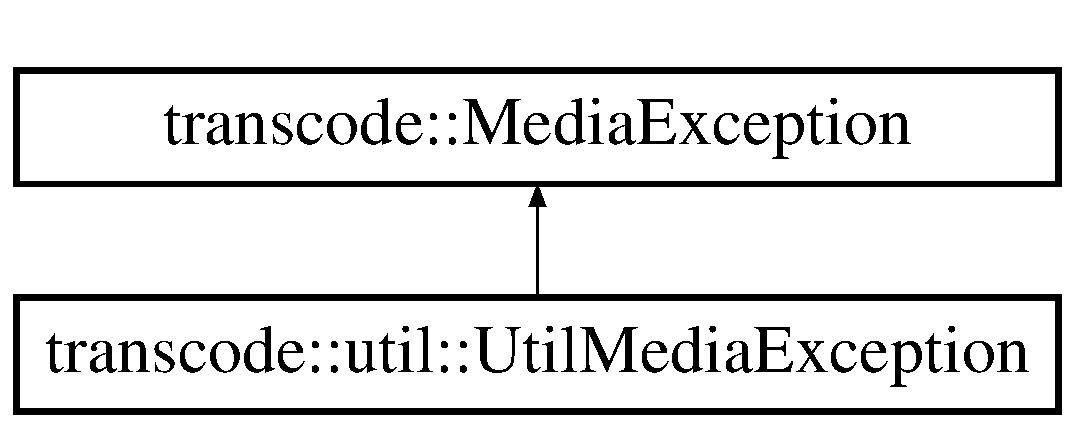
\includegraphics[height=2.000000cm]{classtranscode_1_1util_1_1UtilMediaException}
\end{center}
\end{figure}
\subsection*{Public Member Functions}
\begin{DoxyCompactItemize}
\item 
\hyperlink{classtranscode_1_1util_1_1UtilMediaException_a36ad85f029238d06a530913ead5f67d6}{UtilMediaException} ()  throw ()
\begin{DoxyCompactList}\small\item\em Instantiate an empty \hyperlink{classtranscode_1_1MediaException}{MediaException} object. \item\end{DoxyCompactList}\item 
\hyperlink{classtranscode_1_1util_1_1UtilMediaException_a516da50b349d9850d27054fd4f29db4b}{UtilMediaException} (std::string message)  throw ()
\begin{DoxyCompactList}\small\item\em Instantiate a MediaUtilsException object with the provided message. \item\end{DoxyCompactList}\end{DoxyCompactItemize}


\subsection{Detailed Description}
An exception that is thrown from within the MediaUtils functions. 

Definition at line 48 of file util\_\-media.hpp.



\subsection{Constructor \& Destructor Documentation}
\hypertarget{classtranscode_1_1util_1_1UtilMediaException_a36ad85f029238d06a530913ead5f67d6}{
\index{transcode::util::UtilMediaException@{transcode::util::UtilMediaException}!UtilMediaException@{UtilMediaException}}
\index{UtilMediaException@{UtilMediaException}!transcode::util::UtilMediaException@{transcode::util::UtilMediaException}}
\subsubsection[{UtilMediaException}]{\setlength{\rightskip}{0pt plus 5cm}transcode::util::UtilMediaException::UtilMediaException (
\begin{DoxyParamCaption}
{}
\end{DoxyParamCaption}
)  throw ()\hspace{0.3cm}{\ttfamily  \mbox{[}inline\mbox{]}}}}
\label{classtranscode_1_1util_1_1UtilMediaException_a36ad85f029238d06a530913ead5f67d6}


Instantiate an empty \hyperlink{classtranscode_1_1MediaException}{MediaException} object. 



Definition at line 54 of file util\_\-media.hpp.

\hypertarget{classtranscode_1_1util_1_1UtilMediaException_a516da50b349d9850d27054fd4f29db4b}{
\index{transcode::util::UtilMediaException@{transcode::util::UtilMediaException}!UtilMediaException@{UtilMediaException}}
\index{UtilMediaException@{UtilMediaException}!transcode::util::UtilMediaException@{transcode::util::UtilMediaException}}
\subsubsection[{UtilMediaException}]{\setlength{\rightskip}{0pt plus 5cm}transcode::util::UtilMediaException::UtilMediaException (
\begin{DoxyParamCaption}
\item[{std::string}]{message}
\end{DoxyParamCaption}
)  throw ()\hspace{0.3cm}{\ttfamily  \mbox{[}inline\mbox{]}}}}
\label{classtranscode_1_1util_1_1UtilMediaException_a516da50b349d9850d27054fd4f29db4b}


Instantiate a MediaUtilsException object with the provided message. 


\begin{DoxyParams}{Parameters}
{\em message} & -\/ the message for the new exception. \\
\hline
\end{DoxyParams}


Definition at line 63 of file util\_\-media.hpp.



The documentation for this class was generated from the following file:\begin{DoxyCompactItemize}
\item 
src/main/native/util/util\_\-media.hpp\end{DoxyCompactItemize}

\hypertarget{structtranscode_1_1VideoMetaData}{
\section{transcode::VideoMetaData Struct Reference}
\label{structtranscode_1_1VideoMetaData}\index{transcode::VideoMetaData@{transcode::VideoMetaData}}
}


Struct to hold all the common attributes for a video media type.  




{\ttfamily \#include $<$metadata.hpp$>$}

Inheritance diagram for transcode::VideoMetaData:\begin{figure}[H]
\begin{center}
\leavevmode
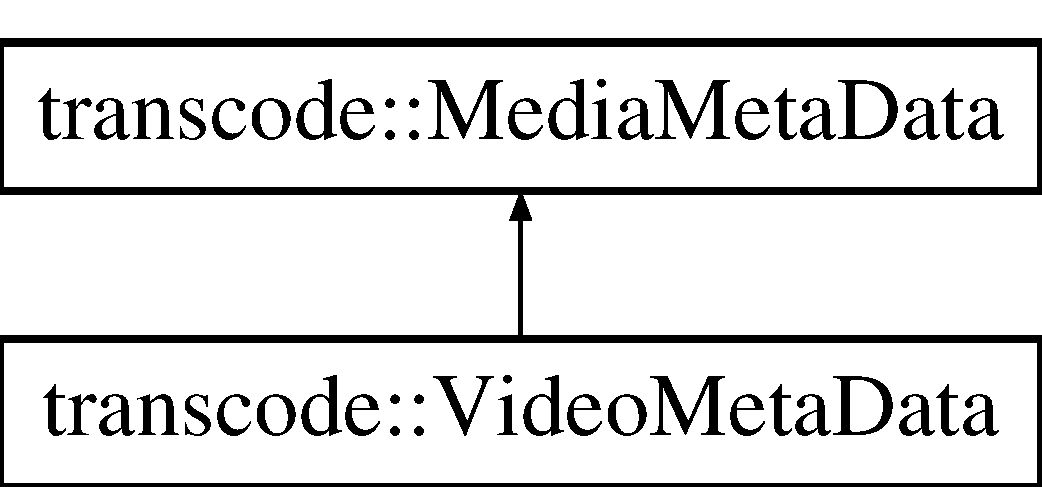
\includegraphics[height=2.000000cm]{structtranscode_1_1VideoMetaData}
\end{center}
\end{figure}
\subsection*{Public Member Functions}
\begin{DoxyCompactItemize}
\item 
\hyperlink{structtranscode_1_1VideoMetaData_ac3e087ef10d6bbb0848a61cc4b8e4b03}{VideoMetaData} (const std::string \&mimeType, const int \&w, const int \&h, const int \&fr)
\begin{DoxyCompactList}\small\item\em Construct a new VideoDetails struct with the provided mimetype, frame width, frame height, and frame rate. \item\end{DoxyCompactList}\end{DoxyCompactItemize}
\subsection*{Public Attributes}
\begin{DoxyCompactItemize}
\item 
\hypertarget{structtranscode_1_1VideoMetaData_af336e4d08b2b6fd357a162f736c858f3}{
int {\bfseries width}}
\label{structtranscode_1_1VideoMetaData_af336e4d08b2b6fd357a162f736c858f3}

\item 
\hypertarget{structtranscode_1_1VideoMetaData_ae9592e63c618a1986efc10533e68cde1}{
int {\bfseries height}}
\label{structtranscode_1_1VideoMetaData_ae9592e63c618a1986efc10533e68cde1}

\item 
\hypertarget{structtranscode_1_1VideoMetaData_a8f5438684245b1079ebd4011638fff7e}{
int {\bfseries frameRate}}
\label{structtranscode_1_1VideoMetaData_a8f5438684245b1079ebd4011638fff7e}

\end{DoxyCompactItemize}


\subsection{Detailed Description}
Struct to hold all the common attributes for a video media type. 

Definition at line 92 of file metadata.hpp.



\subsection{Constructor \& Destructor Documentation}
\hypertarget{structtranscode_1_1VideoMetaData_ac3e087ef10d6bbb0848a61cc4b8e4b03}{
\index{transcode::VideoMetaData@{transcode::VideoMetaData}!VideoMetaData@{VideoMetaData}}
\index{VideoMetaData@{VideoMetaData}!transcode::VideoMetaData@{transcode::VideoMetaData}}
\subsubsection[{VideoMetaData}]{\setlength{\rightskip}{0pt plus 5cm}transcode::VideoMetaData::VideoMetaData (
\begin{DoxyParamCaption}
\item[{const std::string \&}]{mimeType, }
\item[{const int \&}]{w, }
\item[{const int \&}]{h, }
\item[{const int \&}]{fr}
\end{DoxyParamCaption}
)\hspace{0.3cm}{\ttfamily  \mbox{[}inline\mbox{]}}}}
\label{structtranscode_1_1VideoMetaData_ac3e087ef10d6bbb0848a61cc4b8e4b03}


Construct a new VideoDetails struct with the provided mimetype, frame width, frame height, and frame rate. 


\begin{DoxyParams}{Parameters}
{\em mimeType} & -\/ the mimeType for this VideoDetails struct. \\
\hline
{\em w} & -\/ the width of the video image. \\
\hline
{\em h} & -\/ the height of the video image. \\
\hline
{\em fr} & -\/ the average frame rate in frames per second. 0 means a variable framerate. \\
\hline
\end{DoxyParams}


Definition at line 112 of file metadata.hpp.



The documentation for this struct was generated from the following file:\begin{DoxyCompactItemize}
\item 
src/main/native/metadata.hpp\end{DoxyCompactItemize}

\chapter{File Documentation}
\hypertarget{util__ffmpeg_8cpp}{
\section{src/main/native/util/util\_\-ffmpeg.cpp File Reference}
\label{util__ffmpeg_8cpp}\index{src/main/native/util/util\_\-ffmpeg.cpp@{src/main/native/util/util\_\-ffmpeg.cpp}}
}


The implementation for the \hyperlink{util__ffmpeg_8hpp}{util\_\-ffmpeg.hpp} functions.  


{\ttfamily \#include \char`\"{}libavformat/avformat.h\char`\"{}}\par
{\ttfamily \#include \char`\"{}libavcodec/avcodec.h\char`\"{}}\par
{\ttfamily \#include \char`\"{}libavutil/error.h\char`\"{}}\par
{\ttfamily \#include $<$util/util\_\-ffmpeg.hpp$>$}\par
{\ttfamily \#include $<$metadata.hpp$>$}\par
{\ttfamily \#include $<$util/util\_\-standard.hpp$>$}\par
{\ttfamily \#include $<$iostream$>$}\par
{\ttfamily \#include $<$string$>$}\par
{\ttfamily \#include $<$vector$>$}\par
{\ttfamily \#include $<$map$>$}\par
{\ttfamily \#include $<$sstream$>$}\par
{\ttfamily \#include $<$tr1/functional$>$}\par
\subsection*{Classes}
\begin{DoxyCompactItemize}
\item 
class \hyperlink{classtranscode_1_1util_1_1FfmpegSingleton}{transcode::util::FfmpegSingleton}
\begin{DoxyCompactList}\small\item\em A singleton class that provides all the implementations for the FFMPEG functions. \item\end{DoxyCompactList}\end{DoxyCompactItemize}
\subsection*{Namespaces}
\begin{DoxyCompactItemize}
\item 
namespace \hyperlink{namespacehelper}{helper}


\begin{DoxyCompactList}\small\item\em Helper namespace, all helper functions and classes are found here. \item\end{DoxyCompactList}

\item 
namespace \hyperlink{namespacecallback}{callback}


\begin{DoxyCompactList}\small\item\em Callback namespace, all callback functions are found here. \item\end{DoxyCompactList}

\item 
namespace \hyperlink{namespacetranscode}{transcode}


\begin{DoxyCompactList}\small\item\em Transcode namespace, all the top level transcode functions and classes are in this namespace. \item\end{DoxyCompactList}

\item 
namespace \hyperlink{namespacetranscode_1_1util}{transcode::util}


\begin{DoxyCompactList}\small\item\em Util namespace, all the utility functions and classes are found within this namespace. \item\end{DoxyCompactList}

\end{DoxyCompactItemize}
\subsection*{Functions}
\begin{DoxyCompactItemize}
\item 
{\footnotesize template$<$typename T $>$ }\\std::vector$<$ T $>$ \hyperlink{namespacetranscode_1_1util_afaf550997dea9058e5331e14100dcecc}{transcode::util::extractMetaData} (const AVFormatContext $\ast$videoFile, AVMediaType mediatype, std::tr1::function$<$ T(const AVStream \&)$>$ metadataCallback)
\begin{DoxyCompactList}\small\item\em Extract the media meta data of the given type from the libav AVFormatContext struct using the provided get meta data function. \item\end{DoxyCompactList}\item 
std::string \hyperlink{namespacetranscode_1_1util_ac43b28725fca57894665f5775b42111a}{transcode::util::ffmpegErrorMessage} (int errorCode)
\begin{DoxyCompactList}\small\item\em Below is the implementation of the public API functions. \item\end{DoxyCompactList}\item 
AVFormatContext $\ast$ \hyperlink{namespacetranscode_1_1util_a65511e44b87092eba02246dd0a6fe103}{transcode::util::retrieveAVFormatContext} (const std::string \&filePath)  throw (FFMPEGException)
\begin{DoxyCompactList}\small\item\em Retrieve the AVFormatContext for the provided media file. \item\end{DoxyCompactList}\item 
std::vector$<$ SubtitleMetaData $>$ \hyperlink{namespacetranscode_1_1util_a5d54bc962ed8a3ce2d592355e476bcdd}{transcode::util::extractSubtitleDetails} (const AVFormatContext $\ast$videoFile)  throw (FFMPEGException)
\begin{DoxyCompactList}\small\item\em Extract the subtitle details from the provided libav AVFormatContext. \item\end{DoxyCompactList}\item 
std::vector$<$ AudioMetaData $>$ \hyperlink{namespacetranscode_1_1util_a77ca59f993d80e7f19ea20fdc6143222}{transcode::util::extractAudioDetails} (const AVFormatContext $\ast$videoFile)  throw (FFMPEGException)
\begin{DoxyCompactList}\small\item\em Extract the audio detail from the provided libav AVFormatContext. \item\end{DoxyCompactList}\item 
std::vector$<$ VideoMetaData $>$ \hyperlink{namespacetranscode_1_1util_a5755318eb50f620cdc071c7ad23cfff7}{transcode::util::extractVideoDetails} (const AVFormatContext $\ast$videoFile)  throw (FFMPEGException)
\begin{DoxyCompactList}\small\item\em Extract the video detail from the provided libav AVFormatContext. \item\end{DoxyCompactList}\item 
ContainerMetaData \hyperlink{namespacetranscode_1_1util_a38d01175f2cce57e6578e5e46cb385e0}{transcode::util::buildContainerDetail} (const AVFormatContext $\ast$videoFile)  throw (FFMPEGException)
\begin{DoxyCompactList}\small\item\em Build a ContainerDetail struct out of the details in the provided AVFormatContext. \item\end{DoxyCompactList}\item 
void \hyperlink{namespacetranscode_1_1util_ac6274ea5d31808dd2930981770a3946b}{transcode::util::closeCodecs} (AVFormatContext $\ast$videoFile)  throw (FFMPEGException)
\begin{DoxyCompactList}\small\item\em Close any codecs that are related to the provided AVFormatContext. \item\end{DoxyCompactList}\end{DoxyCompactItemize}
\subsection*{Variables}
\begin{DoxyCompactItemize}
\item 
const std::map$<$ CodecID, std::string $>$ \hyperlink{namespacehelper_af150f7275a50533efd1065e69614c1b7}{helper::CODEC\_\-TO\_\-MIMETYPE}
\begin{DoxyCompactList}\small\item\em The map that is used to look up mime types from libav CodecID's. \item\end{DoxyCompactList}\item 
const std::map$<$ std::string, std::string $>$ \hyperlink{namespacehelper_ac0fdcb6f95d20f10e1ee9e9f8c9bd723}{helper::NAME\_\-TO\_\-MIMETYPE}
\begin{DoxyCompactList}\small\item\em The map that is used to look up mime types from libav container names. \item\end{DoxyCompactList}\end{DoxyCompactItemize}


\subsection{Detailed Description}
The implementation for the \hyperlink{util__ffmpeg_8hpp}{util\_\-ffmpeg.hpp} functions. The majority of the implementation is contained within the \{\begin{DoxySeeAlso}{See also}
transcode::utils::FfmpegSingleton\} class. 
\end{DoxySeeAlso}


Definition in file \hyperlink{util__ffmpeg_8cpp_source}{util\_\-ffmpeg.cpp}.


\hypertarget{util__ffmpeg_8hpp}{
\section{src/main/native/util/util\_\-ffmpeg.hpp File Reference}
\label{util__ffmpeg_8hpp}\index{src/main/native/util/util\_\-ffmpeg.hpp@{src/main/native/util/util\_\-ffmpeg.hpp}}
}


The FFMPEG utility functions that provide a simple abstraction of the libav API's.  


{\ttfamily \#include $<$error.hpp$>$}\par
{\ttfamily \#include $<$string$>$}\par
{\ttfamily \#include $<$vector$>$}\par
{\ttfamily \#include $<$map$>$}\par
\subsection*{Classes}
\begin{DoxyCompactItemize}
\item 
class \hyperlink{classtranscode_1_1util_1_1FFMPEGException}{transcode::util::FFMPEGException}
\begin{DoxyCompactList}\small\item\em Exception that is thrown if something goes wrong with the FFMPEG library. \item\end{DoxyCompactList}\end{DoxyCompactItemize}
\subsection*{Namespaces}
\begin{DoxyCompactItemize}
\item 
namespace \hyperlink{namespacetranscode}{transcode}


\begin{DoxyCompactList}\small\item\em Transcode namespace, all the top level transcode functions and classes are in this namespace. \item\end{DoxyCompactList}

\item 
namespace \hyperlink{namespacetranscode_1_1util}{transcode::util}


\begin{DoxyCompactList}\small\item\em Util namespace, all the utility functions and classes are found within this namespace. \item\end{DoxyCompactList}

\end{DoxyCompactItemize}
\subsection*{Functions}
\begin{DoxyCompactItemize}
\item 
std::string \hyperlink{namespacetranscode_1_1util_ac43b28725fca57894665f5775b42111a}{transcode::util::ffmpegErrorMessage} (int errorCode)
\begin{DoxyCompactList}\small\item\em Below is the implementation of the public API functions. \item\end{DoxyCompactList}\item 
AVFormatContext $\ast$ \hyperlink{namespacetranscode_1_1util_a65511e44b87092eba02246dd0a6fe103}{transcode::util::retrieveAVFormatContext} (const std::string \&filePath)  throw (FFMPEGException)
\begin{DoxyCompactList}\small\item\em Retrieve the AVFormatContext for the provided media file. \item\end{DoxyCompactList}\item 
std::vector$<$ SubtitleMetaData $>$ \hyperlink{namespacetranscode_1_1util_a5d54bc962ed8a3ce2d592355e476bcdd}{transcode::util::extractSubtitleDetails} (const AVFormatContext $\ast$videoFile)  throw (FFMPEGException)
\begin{DoxyCompactList}\small\item\em Extract the subtitle details from the provided libav AVFormatContext. \item\end{DoxyCompactList}\item 
std::vector$<$ AudioMetaData $>$ \hyperlink{namespacetranscode_1_1util_a77ca59f993d80e7f19ea20fdc6143222}{transcode::util::extractAudioDetails} (const AVFormatContext $\ast$videoFile)  throw (FFMPEGException)
\begin{DoxyCompactList}\small\item\em Extract the audio detail from the provided libav AVFormatContext. \item\end{DoxyCompactList}\item 
std::vector$<$ VideoMetaData $>$ \hyperlink{namespacetranscode_1_1util_a5755318eb50f620cdc071c7ad23cfff7}{transcode::util::extractVideoDetails} (const AVFormatContext $\ast$videoFile)  throw (FFMPEGException)
\begin{DoxyCompactList}\small\item\em Extract the video detail from the provided libav AVFormatContext. \item\end{DoxyCompactList}\item 
ContainerMetaData \hyperlink{namespacetranscode_1_1util_a38d01175f2cce57e6578e5e46cb385e0}{transcode::util::buildContainerDetail} (const AVFormatContext $\ast$videoFile)  throw (FFMPEGException)
\begin{DoxyCompactList}\small\item\em Build a ContainerDetail struct out of the details in the provided AVFormatContext. \item\end{DoxyCompactList}\item 
void \hyperlink{namespacetranscode_1_1util_ac6274ea5d31808dd2930981770a3946b}{transcode::util::closeCodecs} (AVFormatContext $\ast$videoFile)  throw (FFMPEGException)
\begin{DoxyCompactList}\small\item\em Close any codecs that are related to the provided AVFormatContext. \item\end{DoxyCompactList}\end{DoxyCompactItemize}
\subsection*{Variables}
\begin{DoxyCompactItemize}
\item 
\hypertarget{namespacetranscode_1_1util_a77b6a70cbe66d3c133266d586a923923}{
const std::string {\bfseries transcode::util::UNKNOWN} = \char`\"{}Unknown\char`\"{}}
\label{namespacetranscode_1_1util_a77b6a70cbe66d3c133266d586a923923}

\end{DoxyCompactItemize}


\subsection{Detailed Description}
The FFMPEG utility functions that provide a simple abstraction of the libav API's. 

Definition in file \hyperlink{util__ffmpeg_8hpp_source}{util\_\-ffmpeg.hpp}.


\hypertarget{util__file_8cpp}{
\section{src/main/native/util/util\_\-file.cpp File Reference}
\label{util__file_8cpp}\index{src/main/native/util/util\_\-file.cpp@{src/main/native/util/util\_\-file.cpp}}
}


The implementation for the \hyperlink{util__file_8hpp}{util\_\-file.hpp} functions and classes.  


{\ttfamily \#include $<$util/util\_\-file.hpp$>$}\par
{\ttfamily \#include $<$string$>$}\par
{\ttfamily \#include $<$boost/filesystem.hpp$>$}\par
\subsection*{Namespaces}
\begin{DoxyCompactItemize}
\item 
namespace \hyperlink{namespacetranscode}{transcode}


\begin{DoxyCompactList}\small\item\em Transcode namespace, all the top level transcode functions and classes are in this namespace. \item\end{DoxyCompactList}

\item 
namespace \hyperlink{namespacetranscode_1_1util}{transcode::util}


\begin{DoxyCompactList}\small\item\em Util namespace, all the utility functions and classes are found within this namespace. \item\end{DoxyCompactList}

\end{DoxyCompactItemize}


\subsection{Detailed Description}
The implementation for the \hyperlink{util__file_8hpp}{util\_\-file.hpp} functions and classes. 

Definition in file \hyperlink{util__file_8cpp_source}{util\_\-file.cpp}.


\hypertarget{util__file_8hpp}{
\section{src/main/native/util/util\_\-file.hpp File Reference}
\label{util__file_8hpp}\index{src/main/native/util/util\_\-file.hpp@{src/main/native/util/util\_\-file.hpp}}
}


A file API that provides a simplification of C++ file access.  


{\ttfamily \#include $<$string$>$}\par
{\ttfamily \#include $<$exception$>$}\par
\subsection*{Classes}
\begin{DoxyCompactItemize}
\item 
class \hyperlink{classtranscode_1_1util_1_1FileException}{transcode::util::FileException}
\item 
class \hyperlink{classtranscode_1_1util_1_1File}{transcode::util::File}
\begin{DoxyCompactList}\small\item\em A class that represents a file on the file system, it can be used to access meta data about the file. \item\end{DoxyCompactList}\end{DoxyCompactItemize}
\subsection*{Namespaces}
\begin{DoxyCompactItemize}
\item 
namespace \hyperlink{namespacetranscode}{transcode}


\begin{DoxyCompactList}\small\item\em Transcode namespace, all the top level transcode functions and classes are in this namespace. \item\end{DoxyCompactList}

\item 
namespace \hyperlink{namespacetranscode_1_1util}{transcode::util}


\begin{DoxyCompactList}\small\item\em Util namespace, all the utility functions and classes are found within this namespace. \item\end{DoxyCompactList}

\end{DoxyCompactItemize}


\subsection{Detailed Description}
A file API that provides a simplification of C++ file access. 

Definition in file \hyperlink{util__file_8hpp_source}{util\_\-file.hpp}.


\hypertarget{util__media__ffmpeg_8cpp}{
\section{src/main/native/util/util\_\-media\_\-ffmpeg.cpp File Reference}
\label{util__media__ffmpeg_8cpp}\index{src/main/native/util/util\_\-media\_\-ffmpeg.cpp@{src/main/native/util/util\_\-media\_\-ffmpeg.cpp}}
}


An FFMPEG based implementation of the \hyperlink{util__media_8hpp_source}{util\_\-media.hpp} API.  


{\ttfamily \#include \char`\"{}libavformat/avformat.h\char`\"{}}\par
{\ttfamily \#include \char`\"{}libavcodec/avcodec.h\char`\"{}}\par
{\ttfamily \#include $<$util/util\_\-media.hpp$>$}\par
{\ttfamily \#include $<$metadata.hpp$>$}\par
{\ttfamily \#include $<$error.hpp$>$}\par
{\ttfamily \#include $<$util/util\_\-file.hpp$>$}\par
{\ttfamily \#include $<$util/util\_\-ffmpeg.hpp$>$}\par
{\ttfamily \#include $<$string$>$}\par
{\ttfamily \#include $<$vector$>$}\par
{\ttfamily \#include $<$tr1/functional$>$}\par
\subsection*{Namespaces}
\begin{DoxyCompactItemize}
\item 
namespace \hyperlink{namespacehelper}{helper}


\begin{DoxyCompactList}\small\item\em Helper namespace, all helper functions and classes are found here. \item\end{DoxyCompactList}

\item 
namespace \hyperlink{namespacetranscode}{transcode}


\begin{DoxyCompactList}\small\item\em Transcode namespace, all the top level transcode functions and classes are in this namespace. \item\end{DoxyCompactList}

\item 
namespace \hyperlink{namespacetranscode_1_1util}{transcode::util}


\begin{DoxyCompactList}\small\item\em Util namespace, all the utility functions and classes are found within this namespace. \item\end{DoxyCompactList}

\end{DoxyCompactItemize}
\subsection*{Functions}
\begin{DoxyCompactItemize}
\item 
{\footnotesize template$<$typename T $>$ }\\T \hyperlink{namespacehelper_ac4210385b9f91f63e6a6c73cd4f15935}{helper::extractCheckedMetaData} (const AVFormatContext $\ast$formatContext, std::tr1::function$<$ T(const AVFormatContext $\ast$)$>$ detailsCallback)  throw (transcode::util::UtilMediaException)
\begin{DoxyCompactList}\small\item\em Helper template used to wrap an extract meta data function so that it's exception can be converted to a UtilMediaException. \item\end{DoxyCompactList}\item 
std::vector$<$ SubtitleMetaData $>$ \hyperlink{namespacetranscode_1_1util_a90c8a8e7393c1d9f8db003a2cad1efba}{transcode::util::findSubtitleMetaData} (const std::string \&filePath)  throw (UtilMediaException)
\begin{DoxyCompactList}\small\item\em Find the subtitle meta data for the media file at the provided path. \item\end{DoxyCompactList}\item 
std::vector$<$ AudioMetaData $>$ \hyperlink{namespacetranscode_1_1util_ad4c7b1a0e312ed159481b9ce476aae6f}{transcode::util::findAudioMetaData} (const std::string \&filePath)  throw (UtilMediaException)
\begin{DoxyCompactList}\small\item\em Find the audio meta data for the media file at the provided path. \item\end{DoxyCompactList}\item 
std::vector$<$ VideoMetaData $>$ \hyperlink{namespacetranscode_1_1util_a50b2171ced48530874981579e184cd2f}{transcode::util::findVideoMetaData} (const std::string \&filePath)  throw (UtilMediaException)
\begin{DoxyCompactList}\small\item\em Find the video meta data for the media file at the provided path. \item\end{DoxyCompactList}\item 
ContainerMetaData \hyperlink{namespacetranscode_1_1util_aca52b690775495a84c8f13094d2de8bf}{transcode::util::findContainerMetaData} (const std::string \&filePath)  throw (UtilMediaException)
\begin{DoxyCompactList}\small\item\em Find the container meta data for the media file at the provided path. \item\end{DoxyCompactList}\item 
MediaFileMetaData \hyperlink{namespacetranscode_1_1util_a66d32ba3f1d1db41872f86838109695b}{transcode::util::findMediaFileMetaData} (const std::string \&filePath)  throw (UtilMediaException)
\begin{DoxyCompactList}\small\item\em Find the meta data for the media file at the provided path. \item\end{DoxyCompactList}\end{DoxyCompactItemize}


\subsection{Detailed Description}
An FFMPEG based implementation of the \hyperlink{util__media_8hpp_source}{util\_\-media.hpp} API. 

Definition in file \hyperlink{util__media__ffmpeg_8cpp_source}{util\_\-media\_\-ffmpeg.cpp}.


\hypertarget{util__standard_8hpp}{
\section{src/main/native/util/util\_\-standard.hpp File Reference}
\label{util__standard_8hpp}\index{src/main/native/util/util\_\-standard.hpp@{src/main/native/util/util\_\-standard.hpp}}
}


An API that provided utility functions to help simplify some usages of the STL.  


{\ttfamily \#include $<$map$>$}\par
\subsection*{Namespaces}
\begin{DoxyCompactItemize}
\item 
namespace \hyperlink{namespacetranscode}{transcode}


\begin{DoxyCompactList}\small\item\em Transcode namespace, all the top level transcode functions and classes are in this namespace. \item\end{DoxyCompactList}

\item 
namespace \hyperlink{namespacetranscode_1_1util}{transcode::util}


\begin{DoxyCompactList}\small\item\em Util namespace, all the utility functions and classes are found within this namespace. \item\end{DoxyCompactList}

\end{DoxyCompactItemize}
\subsection*{Functions}
\begin{DoxyCompactItemize}
\item 
{\footnotesize template$<$typename K , typename V $>$ }\\V \hyperlink{namespacetranscode_1_1util_a250303dbe84b229a60d951d9004d4464}{transcode::util::get} (const std::map$<$ K, V $>$ \&map, const K \&key)
\begin{DoxyCompactList}\small\item\em Convenience template to make it easier to get the value out of a constant map. \item\end{DoxyCompactList}\end{DoxyCompactItemize}


\subsection{Detailed Description}
An API that provided utility functions to help simplify some usages of the STL. 

Definition in file \hyperlink{util__standard_8hpp_source}{util\_\-standard.hpp}.


\printindex
\end{document}
